\chapter{Latches, Flip-Flop e memorie}

Fino ad ora abbiamo visto inverter grazie al quale possiamo ottenere tutte le logiche che abbiamo bisogno cambiano il pull-down/up, dunque sappiamo anche implicitamente creare i circuiti combinatori con varie possibili soluzioni.

A questo punto ci resta da vedere come creare gli elementi di memoria, utilizzate nei \textbf{circuiti sequenziali}.

\section{Circuiti sequenziali}

I circuiti sequenziali, come visto in Reti Logiche, sono formati da una rete combinatoria, che sappiamo costruire, e da una parte di memoria che mantiene i valori della rete combinatoria.

\begin{figure}[htbp]
    \centering
    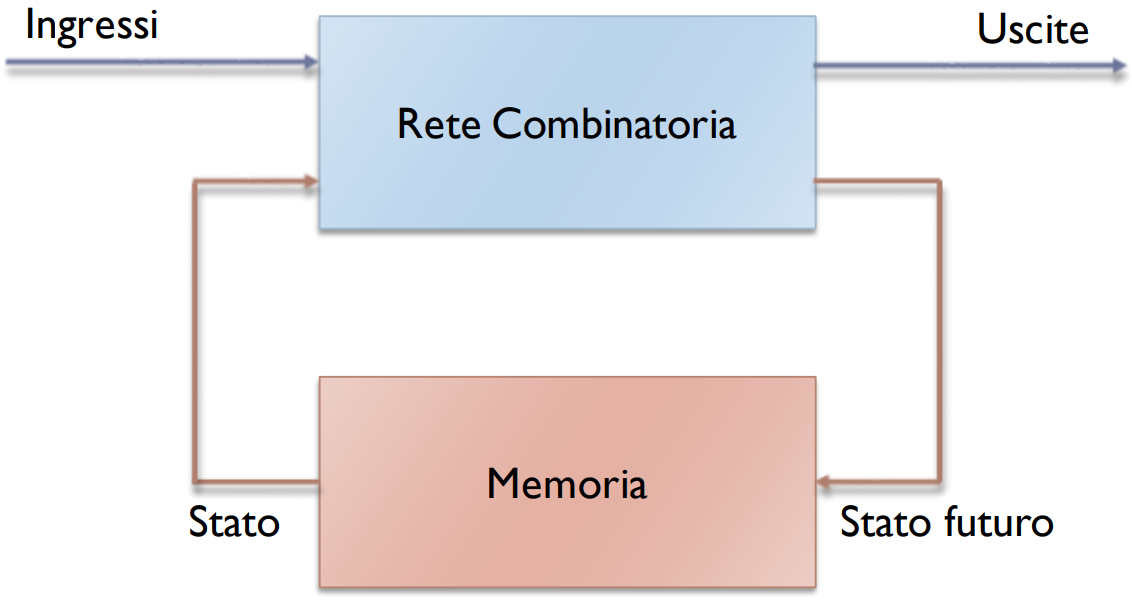
\includegraphics[width=0.5\linewidth]{img/circ_seq.png}
    \caption{Circuito sequenziale}    
\end{figure}

Il problema dunque è quello di mantenere un valore logico. Una primissima soluzione sarebbe quella di sfruttare la memoria insita in un componente elettronico data dal fatto che vi è un dato tempo di propagazione del segnale (ritardo).

Un buffer mantiene un valore al suo interno per un tempo pari al ritardo di propagazione del segnale $t_p$, questo ritardo ovviamente non basta vogliamo memorizzare il valore per molto più tempo. Una soluzione potrebbe essere, sfruttando la logica dinamica, quella di usare i condensatori, i quali però si scarica e si dovrebbe quindi "rinfrescare" il valore di tanto in tanto.

Alcune memorie RAM le utilizzano.

\section{Circuiti bistabili}

Un modo per non perdere il valore all'ingresso è quello di creare un anello tra uscita ed ingresso, così facendo otteniamo il cosiddetto \textbf{loop di feedback}.
\newpage
\begin{figure}[htbp]
    \centering
    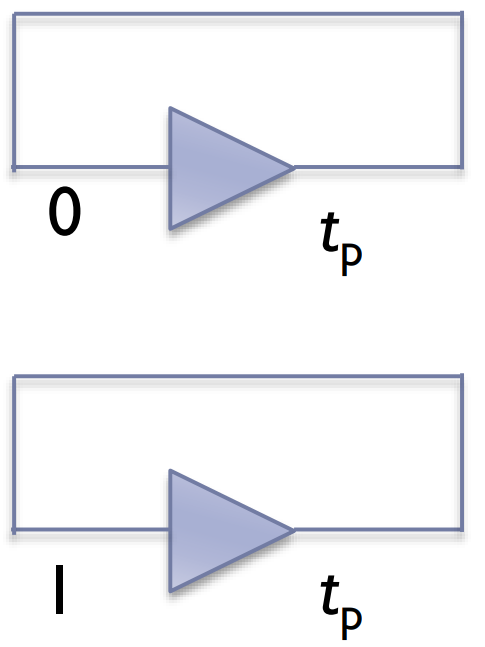
\includegraphics[width=0.25\linewidth]{img/feedback.png}
    
    
\end{figure}

Supponiamo in ingresso ci sia uno 0, se il valore all'ingresso permane almeno per il ritardo di
propagazione, questo sarà mantenuto per almeno un altro
ritardo, e così via.

\paragraph{}
Il circuito è \textbf{stabile}, è stabile sia per uno 0 che per un 1 e si definisce: \textbf{bistabile}.

Per realizzare questo circuito, buffer, basta unire due inverter in cascata.


\subsection{Realizzazione con due inverter}
Il circuito di memoria è normalmente realizzato come due
invertitori in serie



\begin{figure}[htbp]
    \centering
    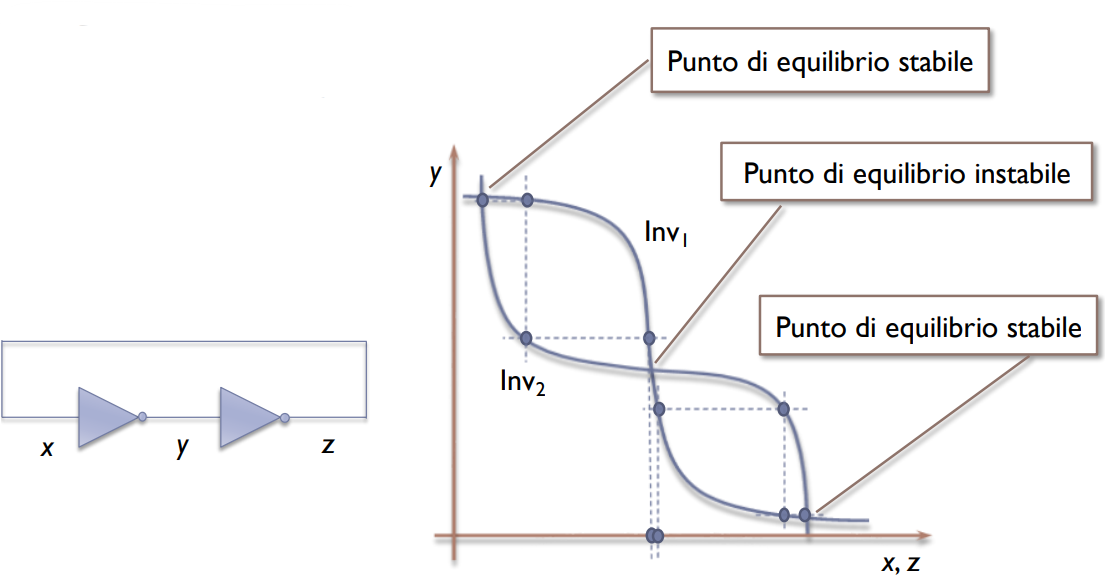
\includegraphics[width=0.75\linewidth]{img/io_buffer.png}
    
    
\end{figure}

Partendo da metà, il circuito si porta ad uno dei due punti stabili. Questo si verificherà sempre in quanto nel circuito vi è sempre del rumore. Il problema è che non sappiamo dove andrà, e men che meno quanto tempo impiega per decidere quale valore preservare!

\paragraph{}

Questo punto è chiamato anche definito come metastabile, ed è utilizzato per creare numeri casuali.

\subsection{Buffer invertente}

Proviamo a fare questo ragionamento anche per un buffer invertente.

\begin{figure}[htbp]
    \centering
    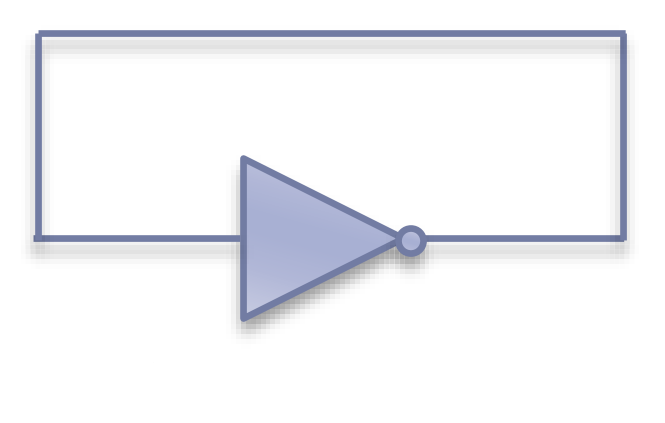
\includegraphics[width=0.25\linewidth]{img/buf_invertente.png}
    \caption{Oscillatore ad anello}
    
\end{figure}

\newpage
Supponiamo ci sia uno 0 all'ingresso, dopo un tempo $t_p$ troviamo un 1 in uscita, questo ritorna all'ingresso e dopo un tempo $t_p$ diventa uno 0 in uscita, che ritorna all'ingresso, e riparte da capo.


Il circuito non è stabile, abbiamo fatto un oscillatore e il periodo di oscillazione è pari a 2 volte $t_p$ utile per generare dei clock. Mettendo una resistenza e condensatore si può regolare la frequenza di oscillazione. In laboratorio questo circuito si può fare utilizzando due inverter per allungare un po' il ritardo, altrimenti capiteremo  nel punto metastabile. 

Attenzione che creando circuiti complessi può capitare che si creino dei feedback, i quali possono creare un circuito oscillante!

\paragraph{}
Anche gli oscillatori a cristalli di quarzo vengono realizzati con un circuito simile a questo.

\section{Elemento di memoria base}

Abbiamo capito che si può usare un circuito bistabile (due inverter in cascata) per memorizzare un bit. Vogliamo anche poter modificare tale valore a piacere in modo da controllare l'uscita.
\paragraph{}

Le porte invertenti hanno un comportamento da inverter.

\subsubsection{EXOR}

Possiamo scegliere se invertire oppure no, cambiando il valore sull'ingresso . Pericoloso: se non invertiamo il circuito diventa instabile.

\begin{figure}[htbp]
    \centering
    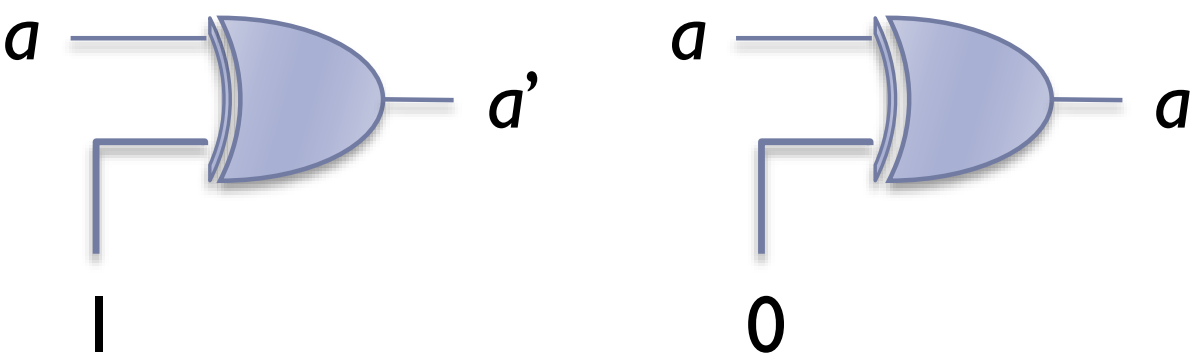
\includegraphics[width=0.5\linewidth]{img/EXOR.png}    
    
\end{figure}

\subsubsection{NOR o NAND}
O invertono o impongono un valore, possiamo dunque decidere cosa fargli fare. Queste porte sembrano soddisfare entrambi i nostri requisiti.

\begin{figure}[htbp]
    \centering
    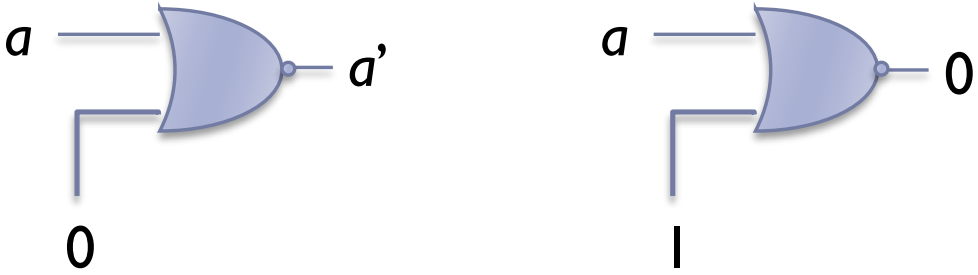
\includegraphics[width=0.5\linewidth]{img/XNOR.png}    
\end{figure}

\newpage
\section{Sostituiamo ciascuno degli inverter con una NOR}

Un ingresso prende il posto dell'ingresso dell'inverter, l'altro lo utilizziamo per controllare l'uscita della porta.

\begin{figure}[htbp]
    \centering
    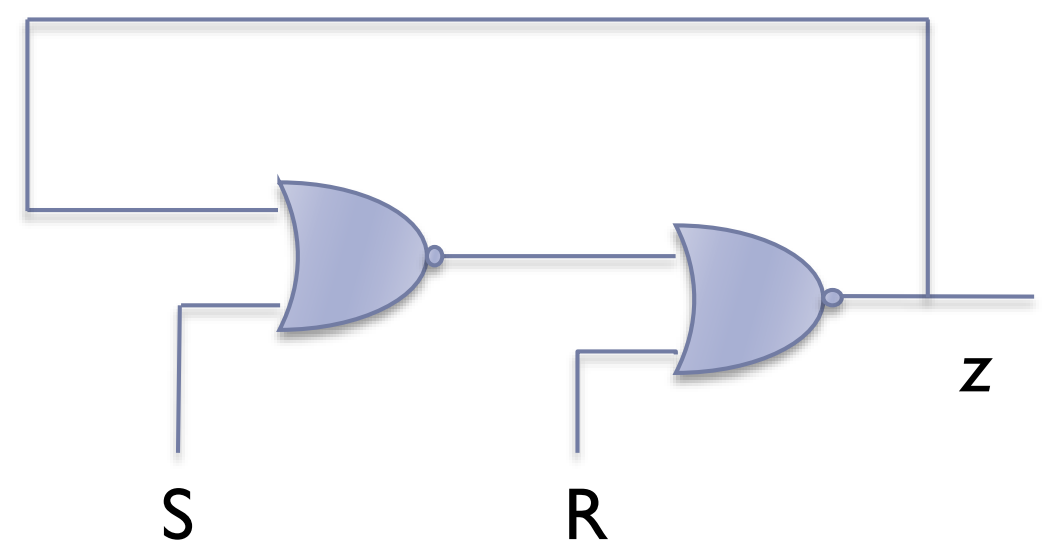
\includegraphics[width=0.4\linewidth]{img/buffer_nor.png}
    
    
\end{figure}

\subsubsection{Uso dei comandi}

\begin{itemize}
    \item Per R = 1 l'uscita si porta a 0
    \item Per S = 1 ed R = 0 l'uscita si porta a 1
    \item Quando S = R = 0 il circuito si comporta come memoria
\end{itemize}


\section{Flip flop SR}

\begin{table}[htbp]
    \centering
    \begin{tabular}{cc|c}
        a & b & NOR\\
        \hline
        0 & 0 & 1\\
        0 & 1 & 0\\
        1 & 0 & 0\\
        1 & 1 & 1\\
    \end{tabular}
    \caption{Tabella di verità NOR}
\end{table}


\subsubsection{NOR incrociati}

Lo stesso circuito si può disegnare in un altro modo:


\begin{figure}[htbp]
    \begin{minipage}[htbp]{0.5\textwidth}
    \centering
        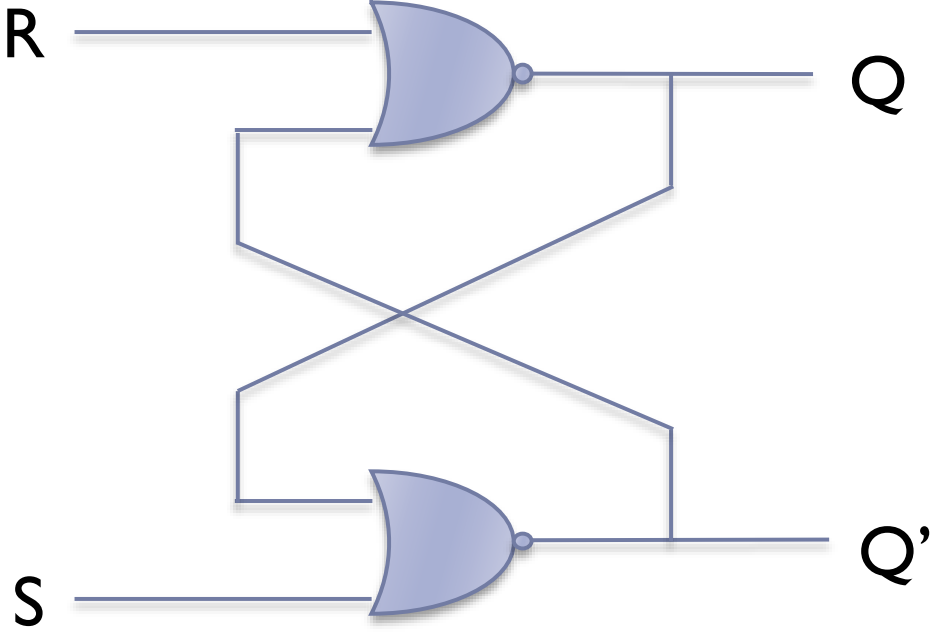
\includegraphics[width=0.8\linewidth]{img/NORRRR.png}
        \caption{Flip Flop SR}
    \end{minipage}
    \begin{minipage}[htbp]{0.5\textwidth}
    \centering

    \begin{tabular}{cc|ccc}
        a & b & Q & Q' & \\
         \hline
        0 & 0 & $Q_{-1}$ & $Q_{-1}'$ & mem\\
        0 & 1 & 0 & 1  & reset\\
        1 & 0 &  1 & 0  & set\\
        1 &  1&  0 & 0   & nd\\
    \end{tabular}
    \caption{Tabella di verità Flip Flop SR}
    
    \end{minipage}
\end{figure}

% \begin{figure}[htbp]
%     \centering
%     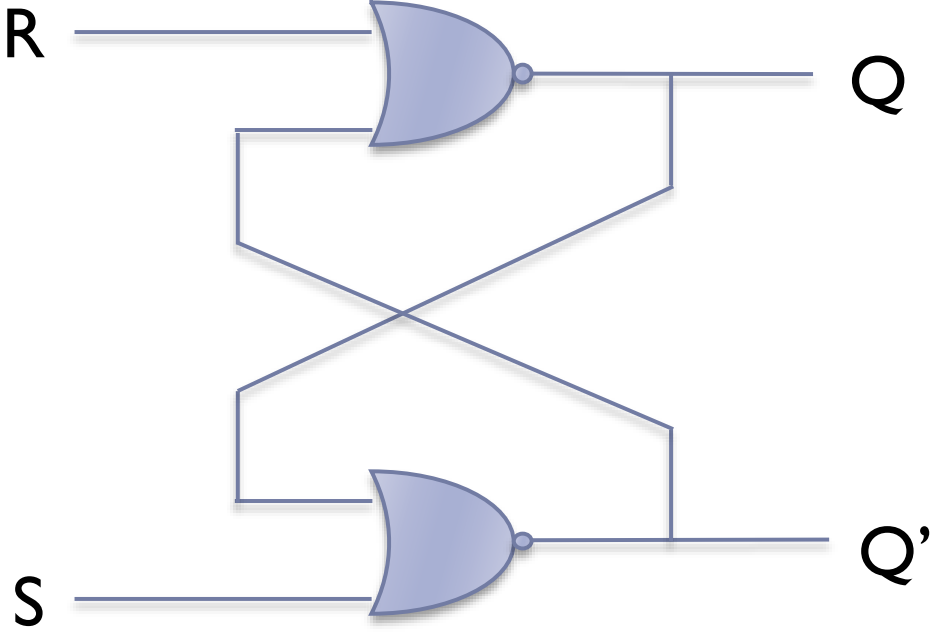
\includegraphics[width=0.4\linewidth]{img/NORRRR.png}

%     \caption{Flip Flop SR}
% \end{figure}

Si evidenzia la struttura simmetrica del circuito.

\begin{equation*}
    Q = (R+ (S+Q)')' = R'(S+Q)
\end{equation*}
\begin{equation*}
    Q = (S+ (R+Q)')' = S'(R+Q)
\end{equation*}


% \begin{table}[htbp]
%     \centering
%     \begin{tabular}{cc|ccc}
%         a & b & Q & Q' & \\
%          \hline
%         0 & 0 & $Q_{-1}$ & $Q_{-1}'$ & mem\\
%         0 & 1 & 0 & 1  & reset\\
%         1 & 0 &  1 & 0  & set\\
%         1 &  1&  0 & 0   & nd\\
%     \end{tabular}
%     \caption{Tabella di verità Flip Flop SR}
% \end{table}


\newpage
\subsection{Funzionamento}

\begin{figure}[htbp]
    \centering
    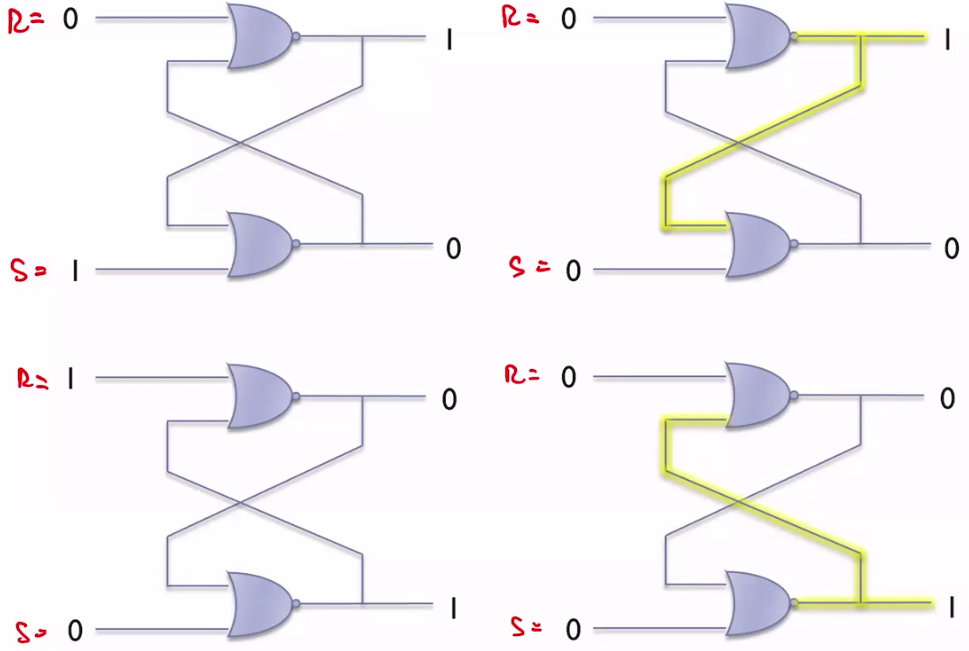
\includegraphics[width=0.5\linewidth]{img/funz.png}
\end{figure}


\subsubsection{Osservazioni}

Le uscite non sono complementari anche se le abbiamo indicate con Q e Q'. Però per S = R = 1 le uscite valgono entrambe 0, ma questa è in realtà una situazione da evitare! Si creerebbero delle \textbf{possibili oscillazioni}.

Supponiamo S = R = 1. Supponiamo che vadano entrambi a 0 contemporaneamente.

Tutti i fili sono a 0, le uscite diventano 1 e quindi di nuovo 0 e così via. 
Il circuito oscilla (0 e 1 si rincorrono,
si arriva a regime se i ritardi non sono
uguali).

\paragraph{}

Oscilla sono in questa situazione con gli ingressi a 1, mettendogli poi uno zero il circuito non sa più dove andare!


\section{Flip flop SR con porte NAND}

Utilizziamo due NAND incrociati.


\begin{equation*}
    Q = (S(RQ)')' = S' + RQ
\end{equation*}
\begin{equation*}
    Q' = (R(SQ)')' = R' + SQ
\end{equation*}

Funziona in modo duale, in questo caso gli ingressi sono attivi bassi.


\begin{figure}[htbp]
    \begin{minipage}[htbp]{0.5\textwidth}
    \centering
        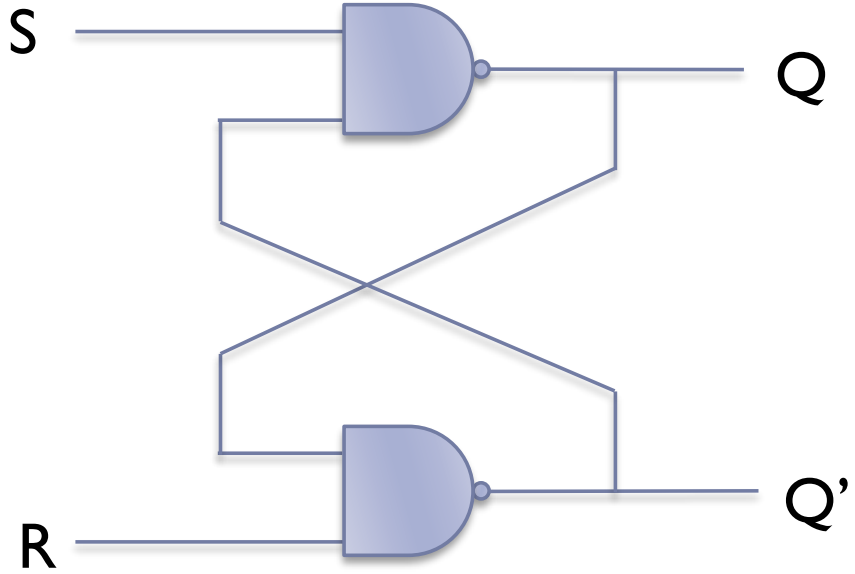
\includegraphics[width=0.8\linewidth]{img/NANDD.png}
        \caption{Flip flop SR con porte NAND}
    \end{minipage}
    \begin{minipage}[htbp]{0.5\textwidth}
    \centering

    \begin{tabular}{cc|ccc}
        S & R & Q' & Q' & \\
        \hline
        0 & 0 & 1 & 1 & nd\\
        0 & 1 & 1 & 0 & set\\
        1 & 0 & 0 & 1 & reset\\
        1 & 1 & $Q_{-1}$ & $Q_{-1}'$ & mem\\
    \end{tabular}
    \caption{Tabella di verità}
    
    \end{minipage}
\end{figure}

% \begin{figure}[htbp]
%     \centering
%     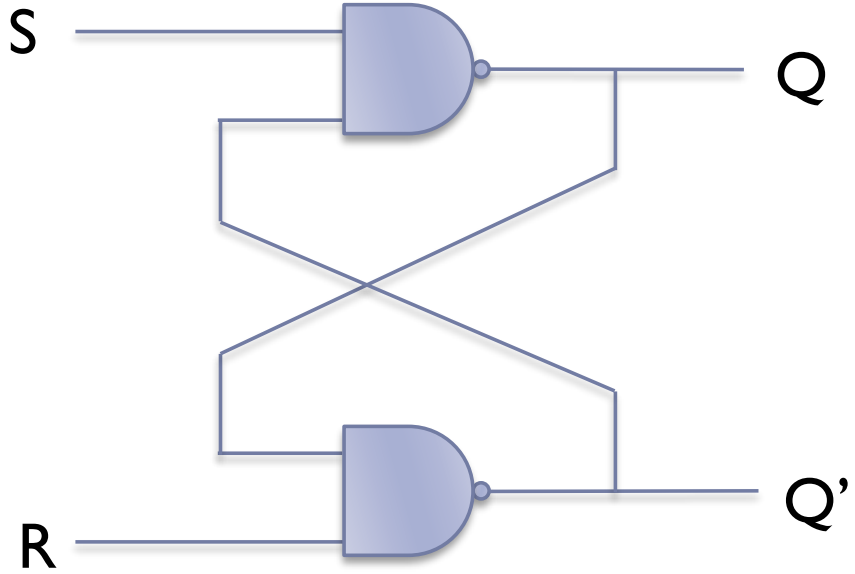
\includegraphics[width=0.4\linewidth]{img/NANDD.png}
%     \caption{Flip flop SR con porte NAND}
% \end{figure}

% \newpage

% \begin{table}
%     \centering
%     \begin{tabular}{cc|ccc}
%         S & R & Q' & Q' & \\
%         \hline
%         0 & 0 & 1 & 1 & nd\\
%         0 & 1 & 1 & 0 & set\\
%         1 & 0 & 0 & 1 & reset\\
%         1 & 1 & $Q_{-1}$ & $Q_{-1}'$ & mem\\
%     \end{tabular}
%     \caption{Tabella di verità di Flip flop SR con porte NAND}
% \end{table}


A questo punto abbiamo realizzato un circuito che riesce ad immagazzinare un bit. A questo punto però vogliamo controllare con un clock quando è il momento di leggere oppure tenere in memoria un dato.

\newpage
\section{Flip flop SR con clock}

Un ingresso di abilitazione controlla quando il flip flop può cambiare di stato, quindi mascheriamo i valori di ingresso con il segnale C!

Il Flip flop è operativo solo quando C = 1, altrimenti è in memoria. Facendo così abbiamo un inversione la quale rende SR attivo alto, funziona in logica positiva.


\begin{figure}[htbp]
    \begin{minipage}[htbp]{0.5\textwidth}
    \centering
        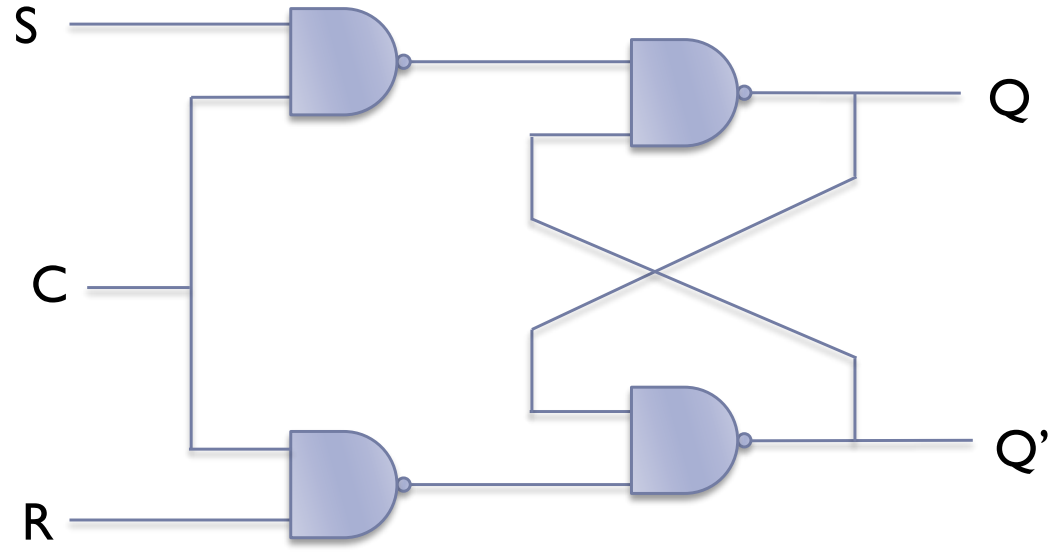
\includegraphics[width=0.9\linewidth]{FFSRC.png}
        \caption{Flip flop SR con porte NAND}
    \end{minipage}
    \begin{minipage}[htbp]{0.5\textwidth}
    \centering

    \begin{tabular}{ccc|ccc}
        C & S & R & Q & Q' & \\
        \hline
        0 & - & - & $Q_{-1}$ & $Q_{-1}'$ & mem\\
        1 & 0 & 0 & $Q_{-1}$ & $Q_{-1}'$ & mem\\
        1 & 0 & 1 & 0 & 1 & reset\\
        1&  1&  0&  1& 0 &set \\
        1 & 1 &  1&  -& - &nd \\
    \end{tabular}
    \caption{Tabella di verità di Flip flop}
    
    \end{minipage}
\end{figure}




% \begin{figure}[htbp]
%     \centering
%     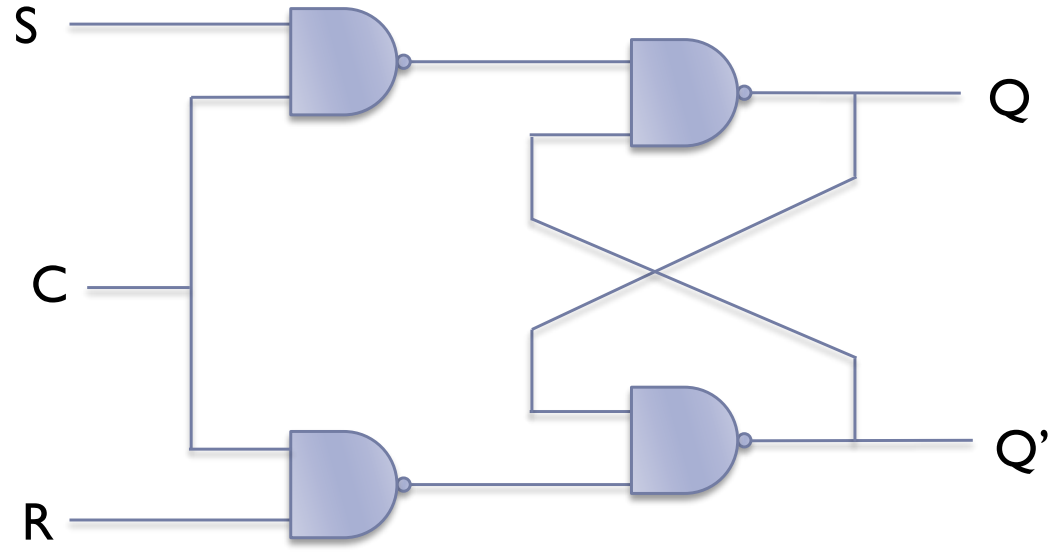
\includegraphics[width=0.5\linewidth]{FFSRC.png}
% \end{figure}


% \begin{table}[htbp]
%     \centering
%     \begin{tabular}{ccc|ccc}
%         C & S & R & Q & Q' & \\
%         \hline
%         0 & - & - & $Q_{-1}$ & $Q_{-1}'$ & mem\\
%         1 & 0 & 0 & $Q_{-1}$ & $Q_{-1}'$ & mem\\
%         1 & 0 & 1 & 0 & 1 & reset\\
%         1&  1&  0&  1& 0 &set \\
%         1 & 1 &  1&  -& - &nd \\
%     \end{tabular}
%     \caption{Tabella di verità di Flip flop SR con porte NAND con clock}
% \end{table}

Nel caso dell'ultima riga abbiamo realizzato proprio quello che prima abbiamo detto che non si doveva fare, infatti quando S e R sono ad uno e il clock passa da 1 a 0 mette il circuito nello stato di instabilità! In questo caso è più semplice di prima portare S ed R a 1, prima era molto più difficile dato che erano due fili separati, ora i due fili sono controllati dal medesimo clock.

\paragraph{}
Per evitare questo disguido si potrebbe aggiungere un inverter: con un solo filo, S, si controlla una porta NAND e con S' si controlla l'altra.
Questa soluzione prende il nome di \textbf{Latch-D} !

\section{Realizzazione ottimizzata}

La realizzazione con NOR o NAND il circuito viene un po' grosso come circuito (17/18 transistori a seconda che sia un flip-flop o un latch).


Una soluzione sarebbe quella di realizzare il circuito con una logica a rapporto.

\paragraph{}
Colleghiamo i due inverter incrociati costruendo un circuito bistabile e proviamo ad imporre un valore ai nodi usando un pull
down che sia più forte del pull up dell'inverter.

\begin{figure}[htbp]
    \centering
    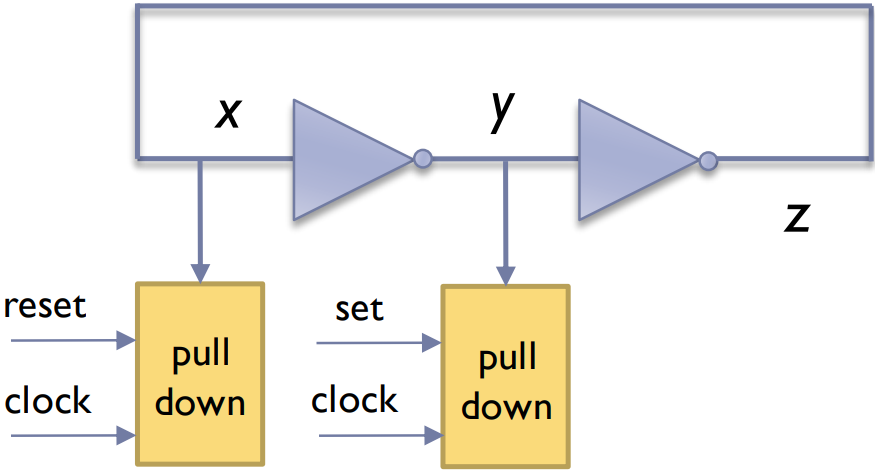
\includegraphics[width=0.45\linewidth]{img/real_ottimiz.png}
\end{figure}


\begin{itemize}
    \item Se tiriamo giù la x, mettiamo l'uscita z a 0 (reset);
    \item Se tiriamo giù la y, mettiamo l'uscita z a 1 (set).
\end{itemize}

Pull down attivo solo quando  il clock è attivo.

\paragraph{}
Il problema della logica a rapporto: il consumo in condizioni statiche, in questo caso però il vantaggio è che una volta importo il valore il pull-down lo posso staccare perché è il feedback che mantiene il valore.

\newpage
\subsection{Schema circuitale}

Combinazione di

\begin{itemize}
    \item[-] Inverter incrociati (M1, M2 – M3, M4)
    \item[-] Doppio pull down (M5, M6 – M7, M8)
    \item[-] Pull down attivi solo per CLK attivo
\end{itemize}


\begin{figure}[htbp]
    \centering
    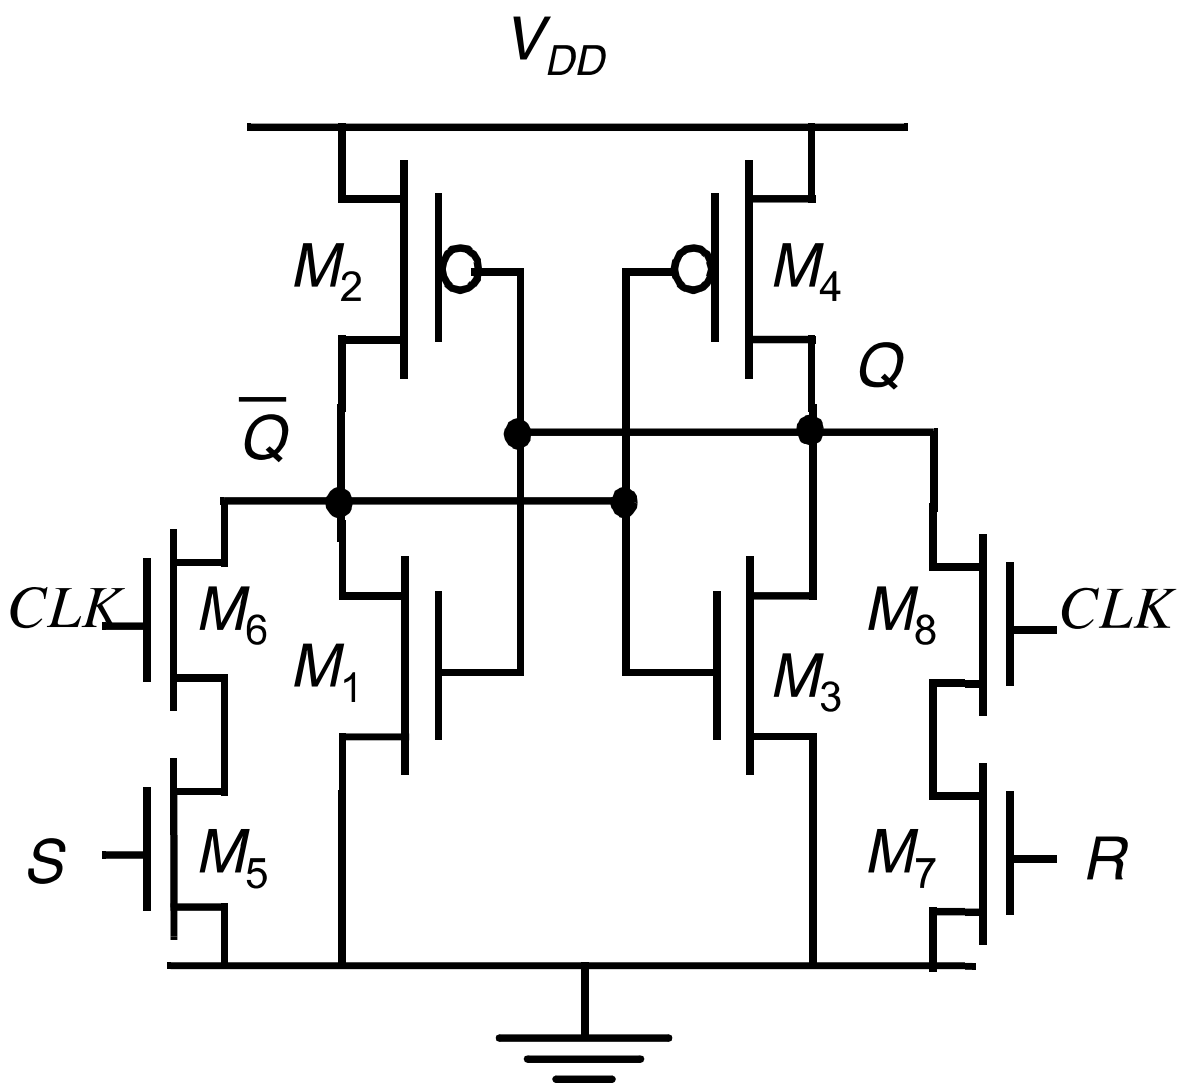
\includegraphics[width=0.4\linewidth]{img/schema_circccc.png}
\end{figure}


\subsection{Funzionamento}

Affinché il circuito funzioni, occorre che i pull-down siano più forti del pull-up. Non deve portare l'uscita a zero, infatti se i due inverter sono simmetrici (soglia di commutazione a $V_{DD}/2$), l'importante che il pull-down deve portare il segnale appena sotto $V_{DD}/2$.

\subsection{Dimensionamento}

Supponiamo che M7 o M8 sia disattivato oppure consideriamoli un unico transistore. L'uscita bassa dell'inverter M4
- M8M7 deve essere minore di $V_{DD}/2$.

Eguagliamo le correnti di M4 e di M87 per $VQ = V_{DD}/2$, ed entrambi i transistori sicuramente in zona triodo.

\begin{itemize}
    \item[] Per M87: $V_{GS} = V_{DD} = 2.5\,V \qquad \qquad V_{DS} = V_{DD}/2 = 1.25\,V$
    \item[] Per M4: $V_{GS} = -V_{DD} = -2.5\,V \qquad \qquad V_{DS} = -V_{DD}/2 = -1.25\,V$
\end{itemize}

\begin{equation*}
    I_{87} = K_n'(\frac{W}{L})_{87}((2.5 - 0.6)1.25 - 0.78125) = 1.6K_n'(\frac{W}{L})_{87}
\end{equation*}

\begin{equation*}
    I_{4} = K_n'(\frac{W}{L})_{4}((-2.5 + 0.6)(-1.25) - 0.78125) = 1.6K_n'(\frac{W}{L})_{4}
\end{equation*}

\begin{equation*}
    K_n'(\frac{W}{L})_{87} = K_p'(\frac{W}{L})_4
\end{equation*}

Assumendo che $(W/L)_4 = 6 $ e $K_n' = 3K_p'$

\begin{itemize}
    \item[] $(W/L)_{87} = 2$
    \item[] $(W/L)_{7} = (W/L)_{8} = 4$
\end{itemize}

\newpage
\section{Ritardo di commutazione}

Il ritardo tra l'attivazione del reset e la commutazione di Q' è Dato dalla somma di 2 componenti.

\begin{itemize}
    \item Il ritardo per portare Q a $V_{DD}/ 2$  dovuto all'inverter pseudo nMOS fatto da M4 e M8 / M7
    \item Il ritardo dovuto all'inverter CMOS fatto dai transistori M2 ed M1
\end{itemize}


\begin{figure}[htbp]
    \centering
    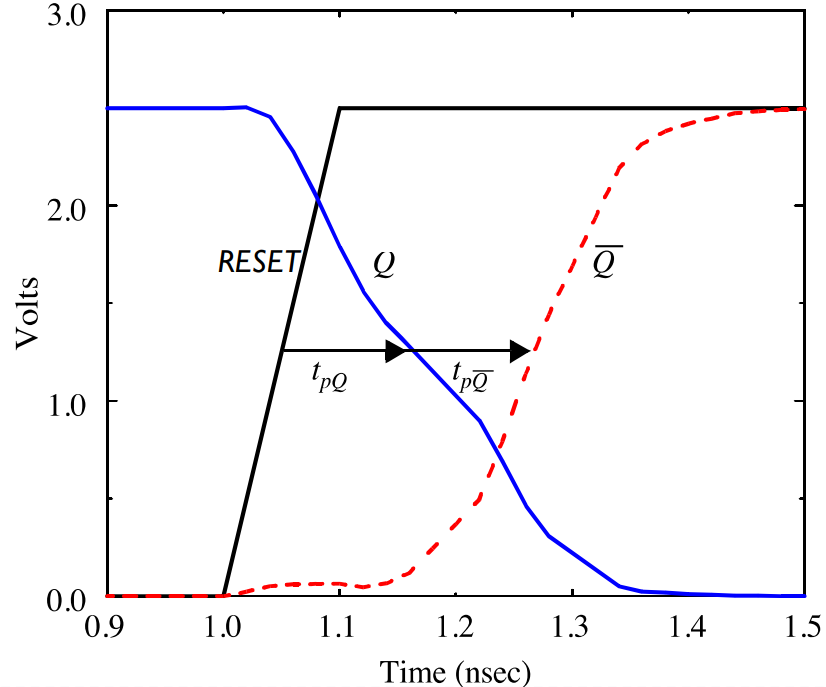
\includegraphics[width=0.5\linewidth]{img/adsvdsv.png}
\end{figure}



\section{Latch basato su multiplexer}

Un altro modo di realizzare il flip flop è quello di usare un multiplexer in retroazione, in VHDL scriveremo:

\begin{equation*}
    \text{q <= d when clk = 1 else q;}
\end{equation*}

\begin{figure}[htbp]
    \centering
    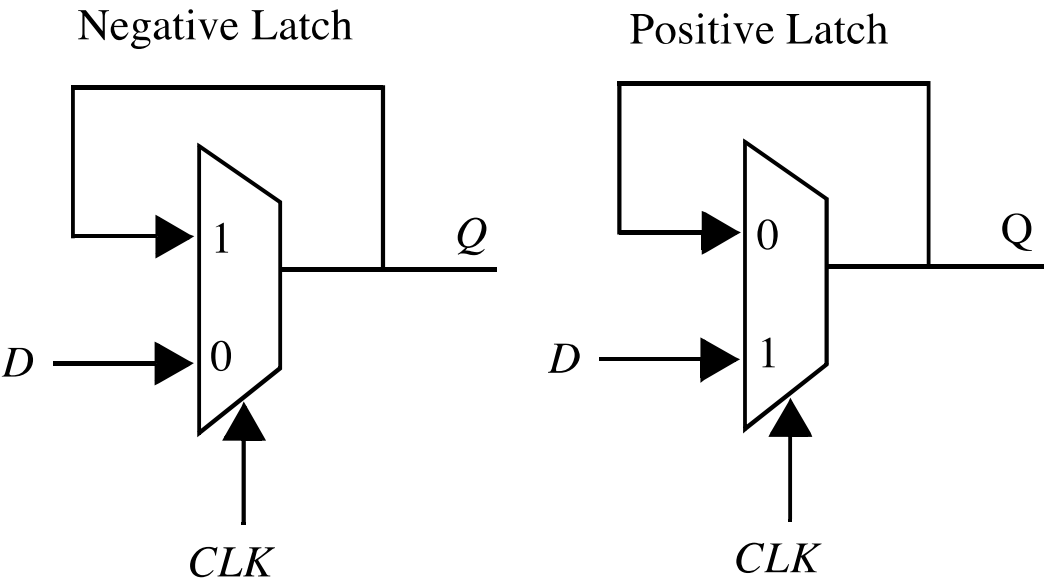
\includegraphics[width=0.5\linewidth]{img/FF_mult.png}
    \caption{Latch basato su multiplexer}
\end{figure}

Questo dispositivo può essere realizzato con logica a transmission gate:

\begin{itemize}
    \item[] Quando CLK = 0 si instaura il feedback
    \item[] Quando CLK = 1 si apre l'anello e si può configurare un nuovo valore
\end{itemize}

\newpage
\begin{figure}[htbp]
    \centering
    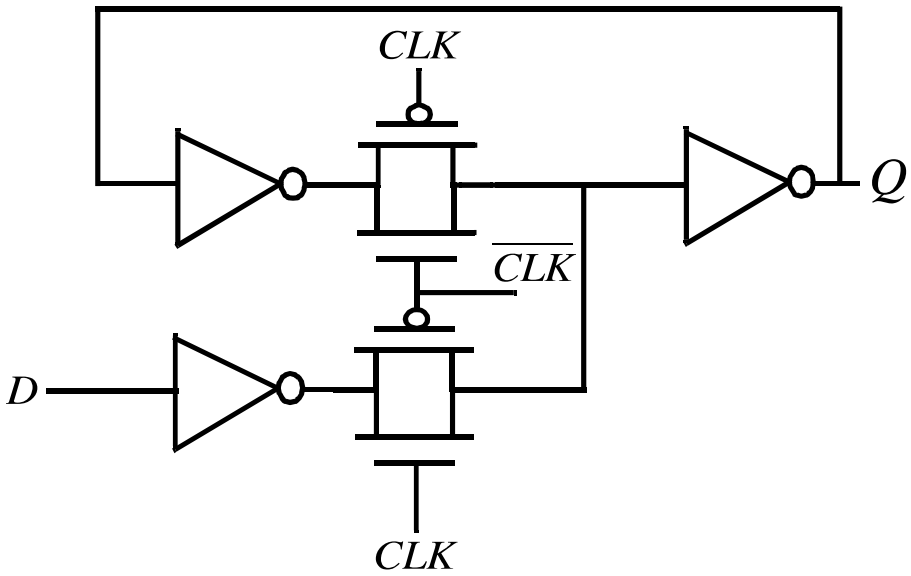
\includegraphics[width=0.4\linewidth]{img/latch_TG.png}
\end{figure}

Non possiamo semplicemente prendere il filo e riportarlo al suo ingresso, bensì dobbiamo inserire la funzione identità utilizzando due inverter i quali provvedono a mantenere un segnale stabile dall'inizio alla fine del canale. 

Un altro inverter è inserito prima del transistore di sotto per disaccoppiare lo switch da chi lo pilotava e abbassare il rumore.
\paragraph{}
Di fatti abbiamo creato un circuito che mantiene il valore, aprendo o chiudendo l'interruttore (transistor superiore) posso decidere se settare o mantenere un bit.

\subsection{Caratteristiche: }

\begin{itemize}
    \item Il funzionamento non dipende più dal rapporto tra le dimensioni dei transistori (il pull-down non deve concorrere con il pull-up);
    \item Dato il punto precedente possiamo creare transistori della dimensione più piccola, da tenere in mente che però porteranno meno corrente (logica lenta);
    \item Il numero di transistori utilizzato è più alto rispetto alla soluzione precedente;
    \item Il carico sul segnale CLK è più alto.
\end{itemize}

Il numero totale di transistori aumenta a 12 transistori contro 8 del circuito precedente.

\paragraph{}
Funzionamento del circuito quando il clk=0, a destra, e quando clk=1, a sinistra.

\begin{figure}[htbp]
    \centering
    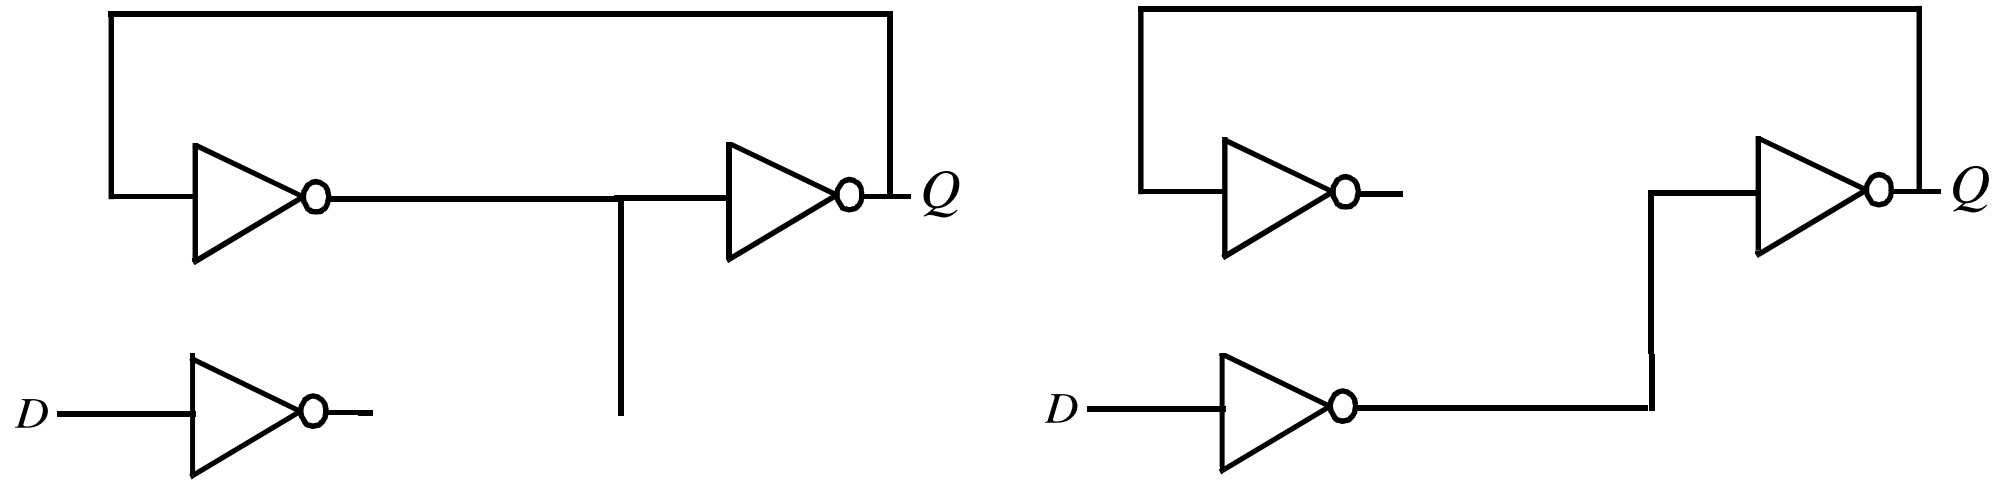
\includegraphics[width=0.65\linewidth]{img/funzionamento_latch_multi.png}
\end{figure}

\newpage
\section{Flip flop di tipo Master Slave}

Nei circuiti sequenziali è molto rischioso usare dei latch sensibili al clock infatti quando il clk=1, il latch è trasparente e nulla vieta al segnale di ingresso di variare provocando errori nella logica combinatoria.

Per risolvere questo problema utilizziamo la soluzione vista a Reti Logiche, due flip flop con clock in cascata.

\begin{figure}[htbp]
    \centering
    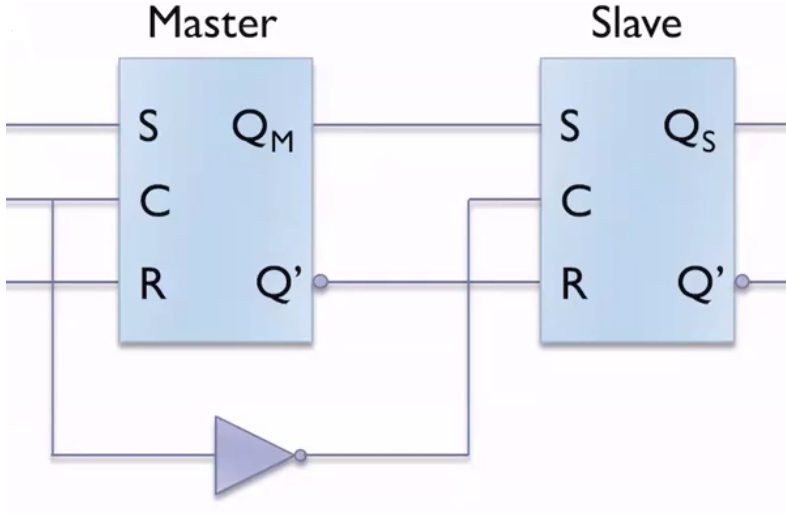
\includegraphics[width=0.5\linewidth]{img/master_slave.png}
\end{figure}

Il primo, detto master, aperto quando il clock è alto; Il secondo, detto slave, aperto quando il clock è basso.
In questo modo non avremo mai un cammino che va dall'ingresso all'uscita.

Ma vi è un cammino indiretto tra ingresso e uscita:
\paragraph{}
\begin{itemize}
    \item[] Quando C = 1 il primo flip flop è aperto e si può impostare il valore di $Q_M$;
    \item[] Quando C esegue la transizione da 1 a 0 il valore di $Q_M$ viene trasferito nel secondo flip flop e sull'uscita $Q_S$;
    \item[] Mentre C = 0 tutto sta fermo perché il primo non è sensibile, e il secondo ha gli ingressi fissi.
\end{itemize}

Vediamo che questo circuito è sensibile al fronte di discesa: falling edge.

\paragraph{}
Una variante del circuito è il \textbf{Flip flip edge triggered}, al posto di metter un flip flop RS come ingresso, utilizziamo un flip flop di tipo D.

\begin{figure}[htbp]
    \centering
    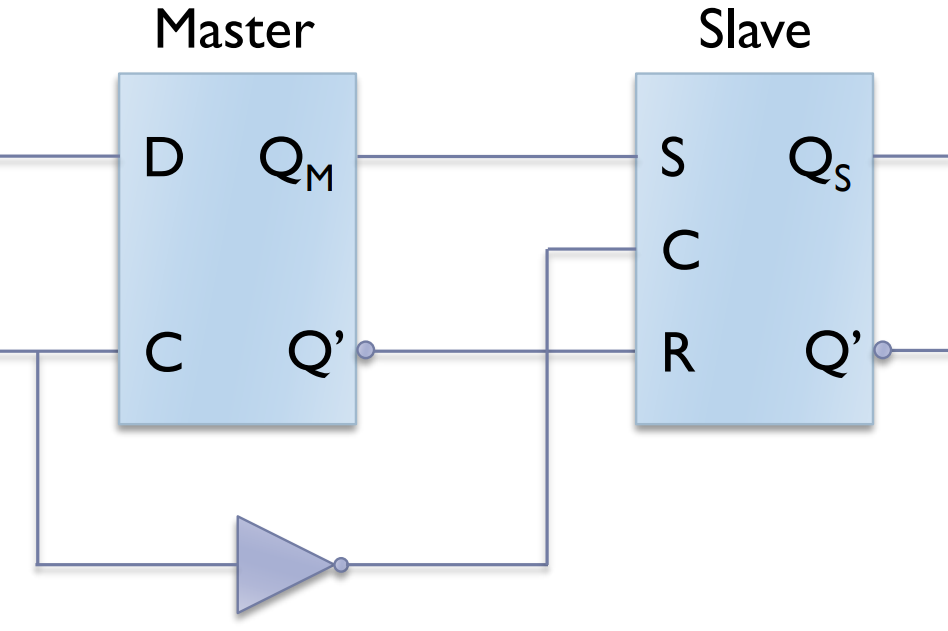
\includegraphics[width=0.5\linewidth]{img/edge_trigg.png}
    \caption{Flip flop edge triggered}
\end{figure}

Il valore di Q è sempre uguale a quello di D nel momento in cui il clock va da 1 a 0. Un solo ingresso D, serve per pilotare S ed R. Il resto funziona in modo analogo a quello precedente.

\newpage
\subsection{Circuito di memoria utilizzando flip flop edge trigger}


\begin{figure}[htbp]
    \centering
    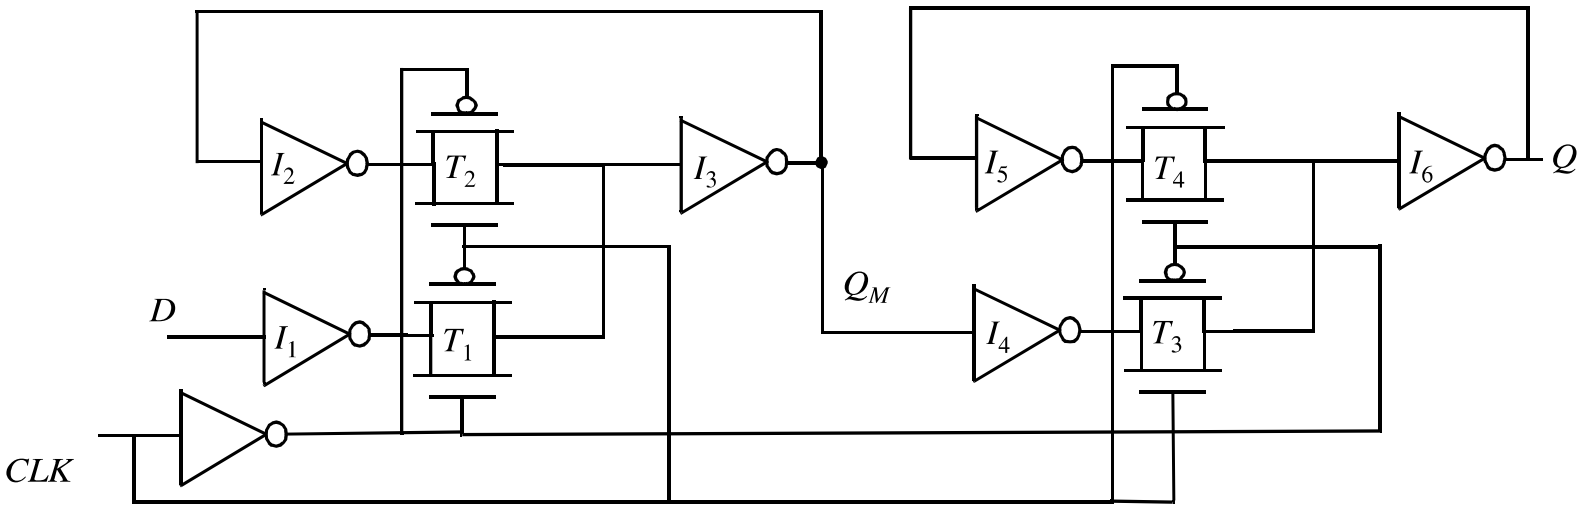
\includegraphics[width=0.65\linewidth]{img/circuito_edge_trigger.png}
\end{figure}

Questo circuito è da caratterizzare in termini di tempistiche, sono due molto importanti:

\begin{itemize}
    \item \textbf{Tempo di set-up}: tempo prima del fronte del clock in cui il segnale D deve essere stabile;
    \item \textbf{Tempo di propagazione}: tempo perché il segnale si propaghi fino all'uscita Q a partire dal fronte del clock;
\end{itemize}

In particolare quando vogliamo settare un valore, set-up, dobbiamo aspettare un tempo per il quale il valore sia passato per $I_3$ fino a $I_2$ altrimenti avremo devi valori che si rincorrono e continuando a cambiare dato i due inverter. Dunque si dovrà inserire il valore da memorizzare un po' prima del fronte attivo del clock in modo tale che il valore si è già propagato almeno fino all'ingresso del transmission gate $T_2$.

\subsection{Tempo di set-up}

Il segnale all'ingresso di $T_2$ deve essere stabile quando arriva il fronte del clock, il segnale D deve passare per $I_1$, $T_1$, $I_3$ e $I_2$. Il tempo di set-up è quindi la somma dei ritardi per 3 inverter e un transmission gate.


\begin{figure}[htbp]
    \centering
    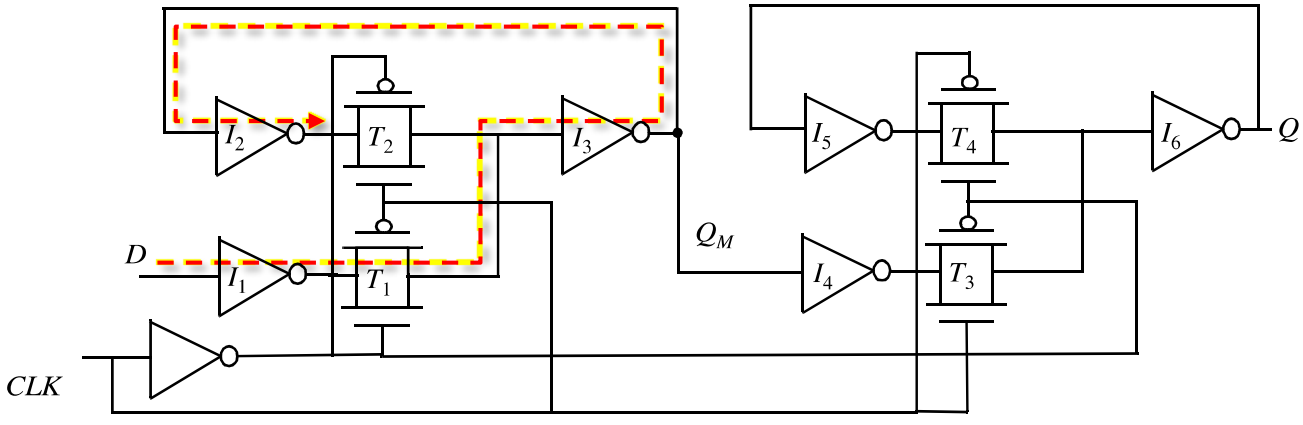
\includegraphics[width=0.6\linewidth]{img/set_up.png}
\end{figure}

\subsection{Tempo di propagazione}

Il segnale all'uscita di $I_4$ è già stabile al fronte, perché
equivale a quello di $I_2$
che deve essere stabile per
soddisfare il tempo di set-up.

Il ritardo è allora dovuto solo a $T_3$ e $I_6$. Tempo di propagazione uguale alla somma dei ritardi per un
transmission gate e un inverter


\begin{figure}[htbp]
    \centering
    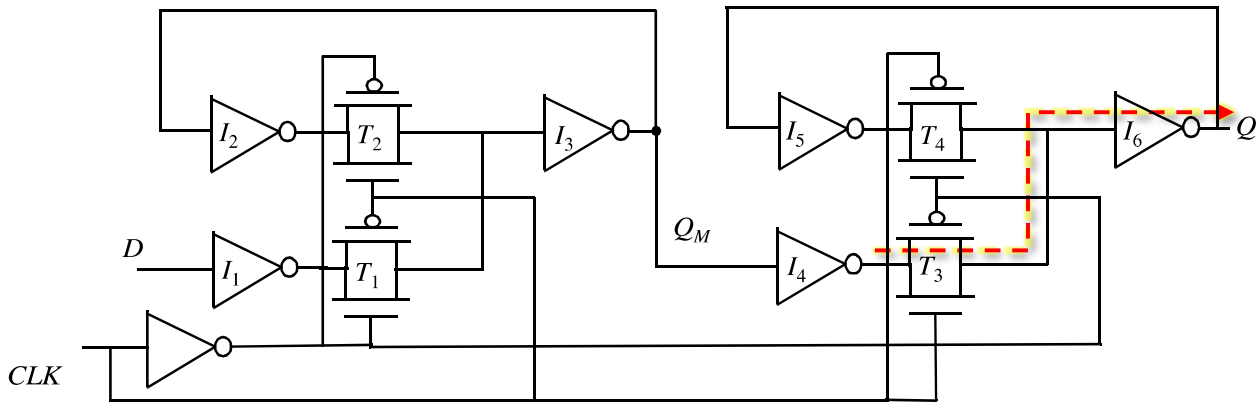
\includegraphics[width=0.63\linewidth]{img/prop.png}
\end{figure}

Contando tutti i transistori il circuito possiede 22 transistori, numero abbastanza elevato, infatti si può fare di meglio.

\newpage
\section{Alternative realizzatile}

Nei circuiti si vuole sempre minimizzare le dimensioni, questo lo si può fare rimuovendo componenti non strettamente necessari al circuito. 

\subsection{Rimuoviamo il transmission gate sul feedback}
Rimuovendo il transmission gate sul feedback avremo che:

\begin{itemize}
    \item Meno transistori caricano il clock;
    \item Ora però chi pilota D assieme al transmission gate T1 deve pilotare più forte di $I_2$;
    \item Occorre dimensionare correttamente i transistori;
    \item Anche $I_4$ deve essere debole, oppure potrebbe influenzare lo stato del primo latch!
\end{itemize}

Ricadiamo in una logica a rapporto! Per questo ci deve essere una comunicazione tra chi produce la cella e chi la deve utilizzare.

\begin{figure}[htbp]
    \centering
    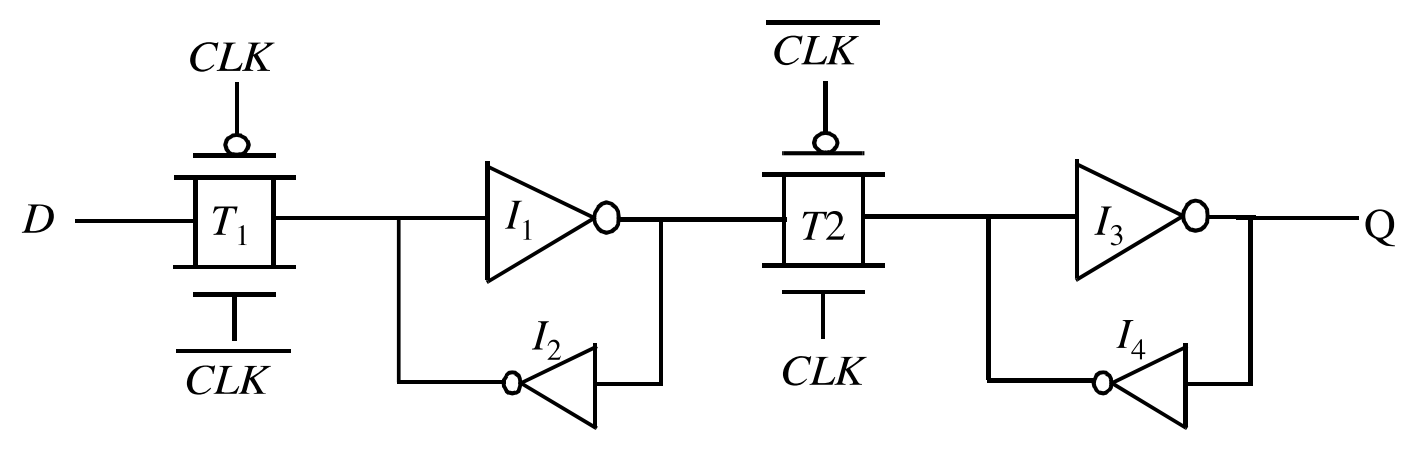
\includegraphics[width=0.6\linewidth]{img/alternativa.png}
\end{figure}

\subsection{Sostituire i transmission gate con pass transistor}

In questo caso il problema è che verrà degradano il livello dei segnali, aumentano i consumi.


\begin{figure}[htbp]
    \centering
    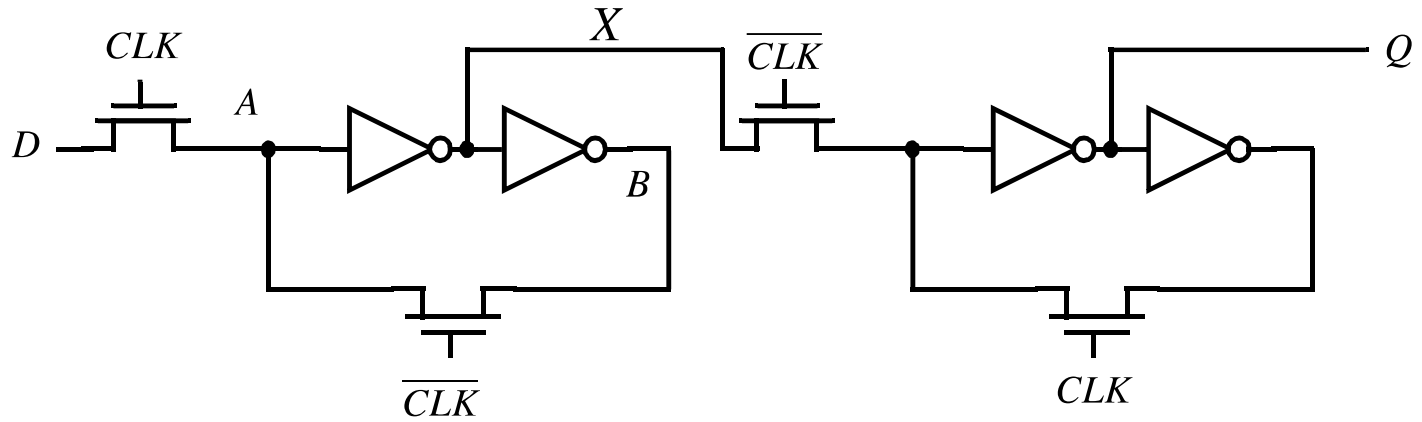
\includegraphics[width=0.6\linewidth]{img/alternativa2.png}
\end{figure}

Uno svantaggio di utilizzare la logica a pass transistor con un inverter è che vi è un consumo statico di corrente. Questo è dovuto al fatto che l'inverter viene pilotato con una tensione che si trova in mezzo, e non agli estremi della tensione di lavoro.

\begin{figure}[htbp]
    \centering
    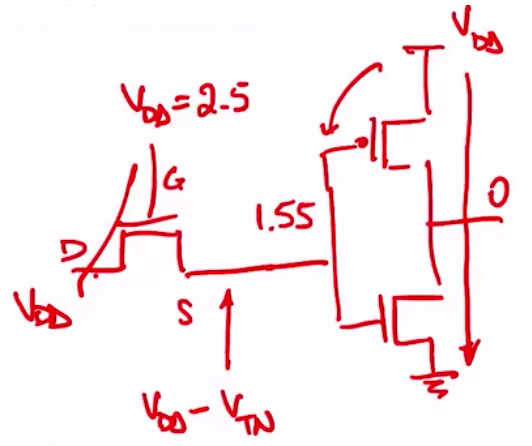
\includegraphics[width=0.35\linewidth]{img/problema_pass.png}
\end{figure}

\newpage
\subsection{Usare logica dinamica}

Frequenza di commutazione deve essere sufficientemente alta altrimenti la capacità si scarica. Questo può essere utilizzato anche come circuito di campionamento.

\begin{figure}[htbp]
    \centering
    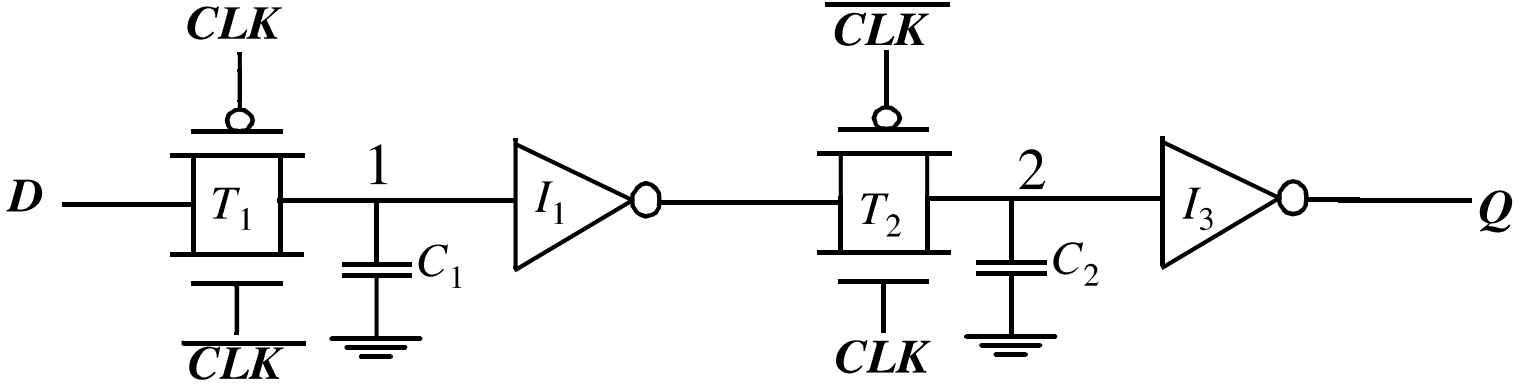
\includegraphics[width=0.7\linewidth]{img/alternatva3.png}
\end{figure}

Da notare che $C_1$ e $C_2$ non ci sono, bensì è la raffigurazione della capacità dell'ingresso dei due transistori dell'inverter.
 

\newpage
\chapter{Memorie RAM}

La memoria non è molto diversa da un flip-flop, la differenza è che solitamente si vogliono memorizzare miliardi di bit ($10^9$ GB) e la vogliamo molto veloce.

La memoria è un insieme di latch strutturati su una matrice quadrata. 


\begin{figure}[htbp]
    \centering
    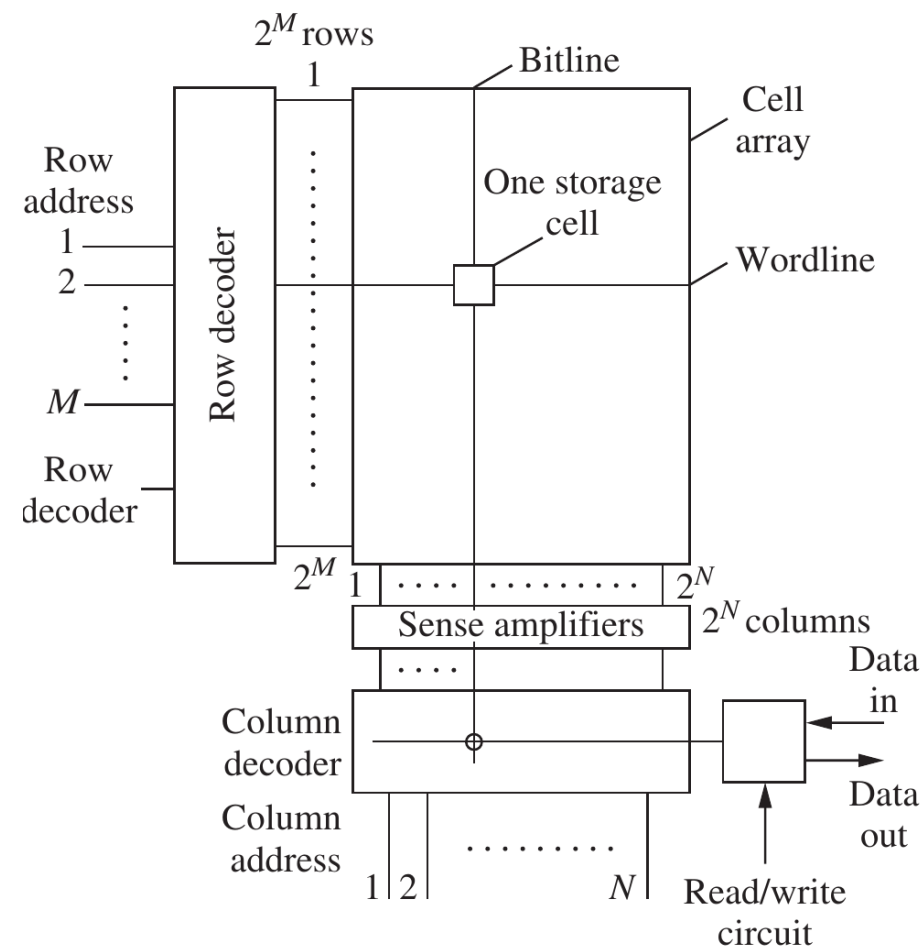
\includegraphics[width=0.5\linewidth]{img/ram.png}
    \caption{RAM}
\end{figure}

Un decoder seleziona la riga
(\textbf{wordline}) della cella desiderata
usando metà dell'indirizzo, vengono lette tutte le celle della
riga selezionata, i sense amplifier amplificano e
talvolta ripristinano i valori nelle
celle lette. Infine un multiplexer seleziona la colonna
(\textbf{bitline}) della cella desiderata
usando l'altra metà dell'indirizzo.


La lettura di un intera riga non fa perdere molto tempo in quanto avviene in parallelo, potrebbe essere però uno spreco di corrente. Questo spreco normalmente non vi è in quanto se si accede ad una posizione di memoria solitamente si vogliono pure leggere i dati contenuti negli indirizzi successivi i quali probabilmente si troveranno proprio sulla stessa riga. In questo modo posso direttamente leggere la colonna senza leggere ancora la riga, con il solo vantaggio di andare più veloci.

\paragraph{Tecniche di programmazione}
In C/C++, e probabilmente anche in molti altri linguaggi, il compilatore ottimizza il codice scrivendo in celle adiacenti il contenuto delle strutture dati come ad esempio le liste.
\paragraph{}
Un esempio di codice non ottimo è utilizzare una struct Punto per memorizzare le coordinate x,y. Infatti in memoria verranno memorizzati tante coordinate in questo modo: XYXYXYXYX. Questo non è ottimo, soprattutto per calcoli paralleli fatti dalle GPU, se si vuole leggere solo il valore di una variabile, infatti la cache richiederà alla DDR celle successive Y anche se queste non verranno utilizzate per il calcolo.

\newpage
\section{Cella statica - la cache}
Le celle di memoria sono sostanzialmente dei latch, la cella statica non viene utilizzata per la costruzione delle DDR, perché troppo grossa, bensì viene utilizzata per la memoria cache in quanto è più veloce per via del suo funzionamento.
\paragraph{}
Il suo funzionamento altro non è che il solito loop tra i due inverter incrociati con controllo di accesso.


\begin{figure}[htbp]
    \centering
    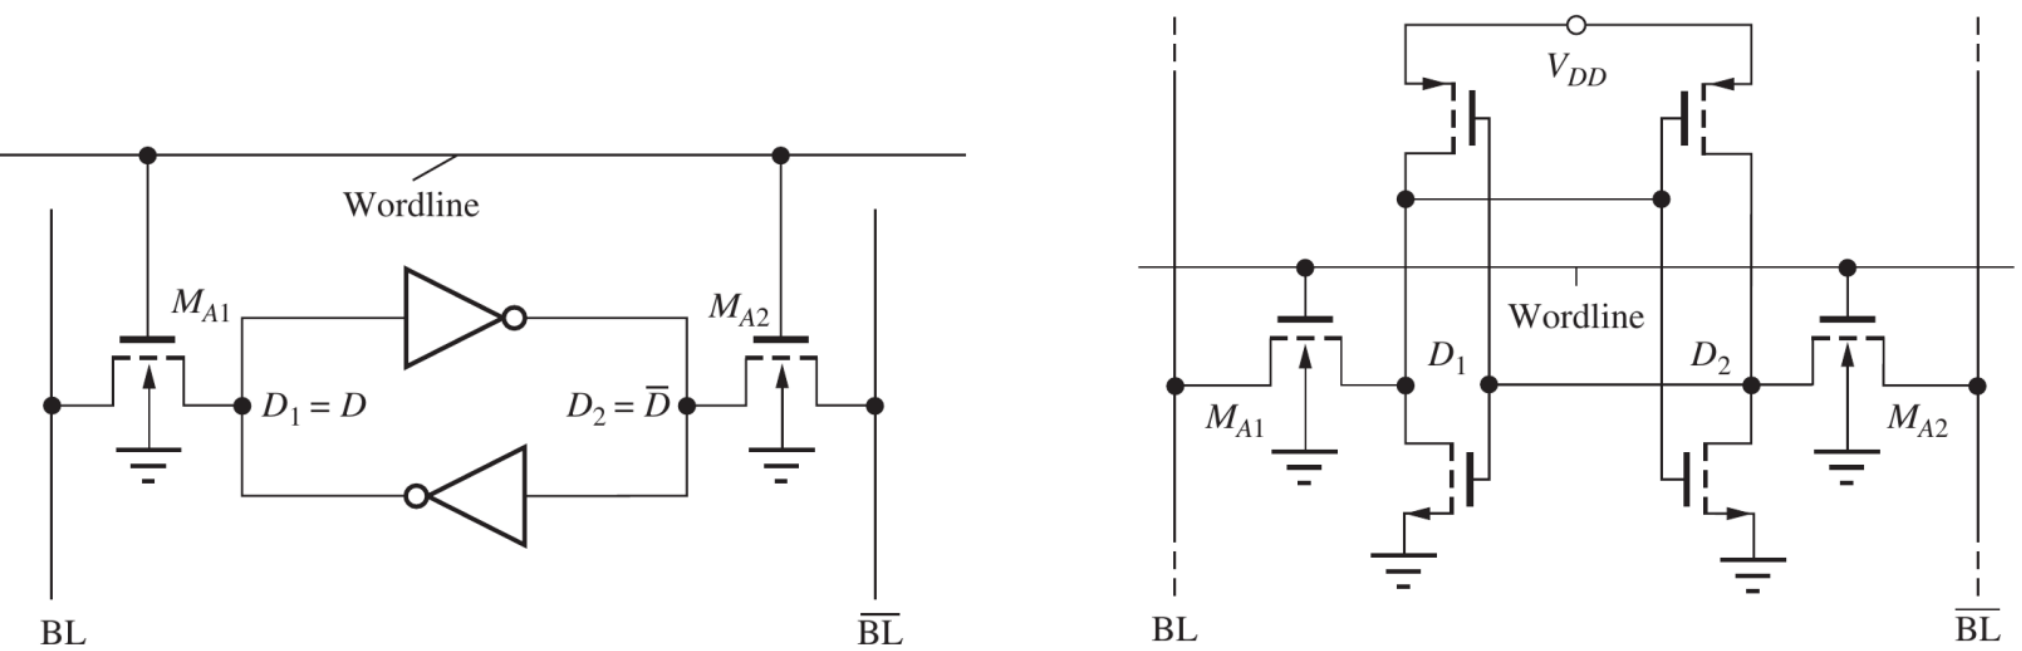
\includegraphics[width=0.7\linewidth]{img/cache.png}
    \caption{Schema circuitale cache}
\end{figure}

L'unica cosa che è un po' diversa nell'accesso a una cella di memoria è proprio il modo in cui cambiamo il valore che è contenuto nella cella. In questo caso utilizziamo un metodo definito \textbf{bilanciato} o \textbf{differenziale}: accesso, lettura, di Q e Q' tramite pass transistor $M_{A1}$ e $M_{A2}$. La wordline, generata dal controllore di riga, attiva l'accesso controllando il gate dei transistori.

\paragraph{}
Le linee che consentono di accedere alla lettura e scrittura di una cella viene chiamata \textbf{bitline}. Ogni colonna ha una coppia di bitline, questo è conveniente per essere veloci a determinare il valore della cella osservando la differenza di valori tra BL e BL' utilizzando il \textbf{sense amplifier}.


\subsection{Lettura della cella}
Le bitline in lettura vengono precaricate a metà della tensione di funzionamento $V_{DD}/2 = 1.5 V$, mentre la wordline è ancora
disattivata. Si potrebbe lasciarle flottanti con il valore precedente, ma si rischia di
andare a scrivere invece di leggere.

A questo punto quando la wordline si attiva, le bitline sono flottanti e se guardo la \textbf{differenza} tra i due transistori vedo subito da che parte sta andando il cambiamento dei valori, e il sense amplifier lo nota e trasmette subito il valore al chiamante.

\paragraph{Esempio: } Supponiamo $D_1 = 0$ V e $D_2 = 3 V$


\begin{figure}[htbp]
    \centering
    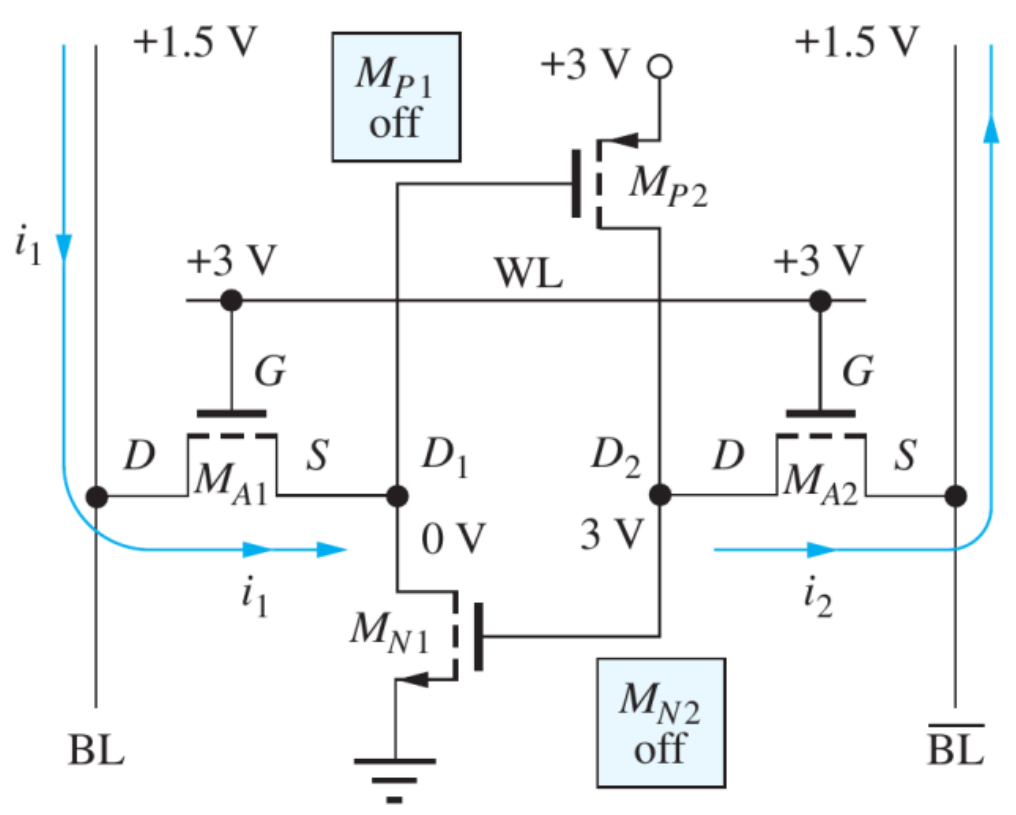
\includegraphics[width=0.4\linewidth]{img/cache1.png}
    \caption{Cella 6-T}
\end{figure}

$M_{A1}$ in zona triodo, $M_{A2}$ in saturazione. $D_1$ tende a salire, $D_2$ tende a scendere. I transistori sono dimensionati in modo tale da
evitare che $D_1$ salga troppo, e si inverta il valore memorizzato!

BL scende, e BL' sale, a questo punto il sense amplifier porta velocemente BL a 0 e BL' a 3 V e termina la lettura.


\subsection{Scrittura della cella}

Si pilotano le bitline con il valore desiderato. 

Supponiamo di voler scrivere 0 quando prima c'era memorizzato un 1, nel caso in cui volessimo scrivere lo stesso valore contenuto già nella cella non succederebbe nulla. $M_{A1}$ è in saturazione e scarica il nodo $D_1$, $M_{A2}$ è anche in saturazione, e fa salire $D_2$ verso $V_{DD} – V_{TN}$, quando $D_2$ supera $D_1$, il feedback positivo fa cambiare il valore nella cella.

\paragraph{NOTA:} Le celle che pilotano le bitline
devono essere dimensionate in
modo da vincere contro gli inverter
della cella, bisogna portare il valore oltre il punto di equilibrio instabile.


\paragraph{}
Questa cella funziona molto bene, ha consumi molto bassi dato che se non cambia nulla il consumo statico è zero, i tempi di accesso sono molto rapidi date le relative alte correnti che scorrono e sono dotate di un sense amplifier che aumenta notevolmente la loro già ottima velocità.

Il problema principale è che sono grosse dati i 6 transistori.

\section{Cella RAM dinamica}

A questo punto potremmo pensare di utilizzare la logica dinamica e salvare il valore in un condensatore, in questo caso vero, creato all'interno del silicio.

Questo circuito è molto semplice, tramite la bitline si accede a un transistor il quale carica o scarica la capacità posta sull'altro terminale. Questo condensatore, essendo che deve essere piccolo per avere determinate velocità, nel giro di pochi millisecondi si scarica e dunque il controllore della RAM deve "rinfrescare" i valori per mantenerli invariati, ovvero li legge e li riscrive.

\paragraph{}
Durante questa operazione di \textbf{refresh} la RAM non è accessibile. Ecco perché non può essere usata come cache, quest'ultima deve essere sempre disponibile, deve rispondere ad un ciclo di clock.


\begin{figure}[htbp]
    \centering
    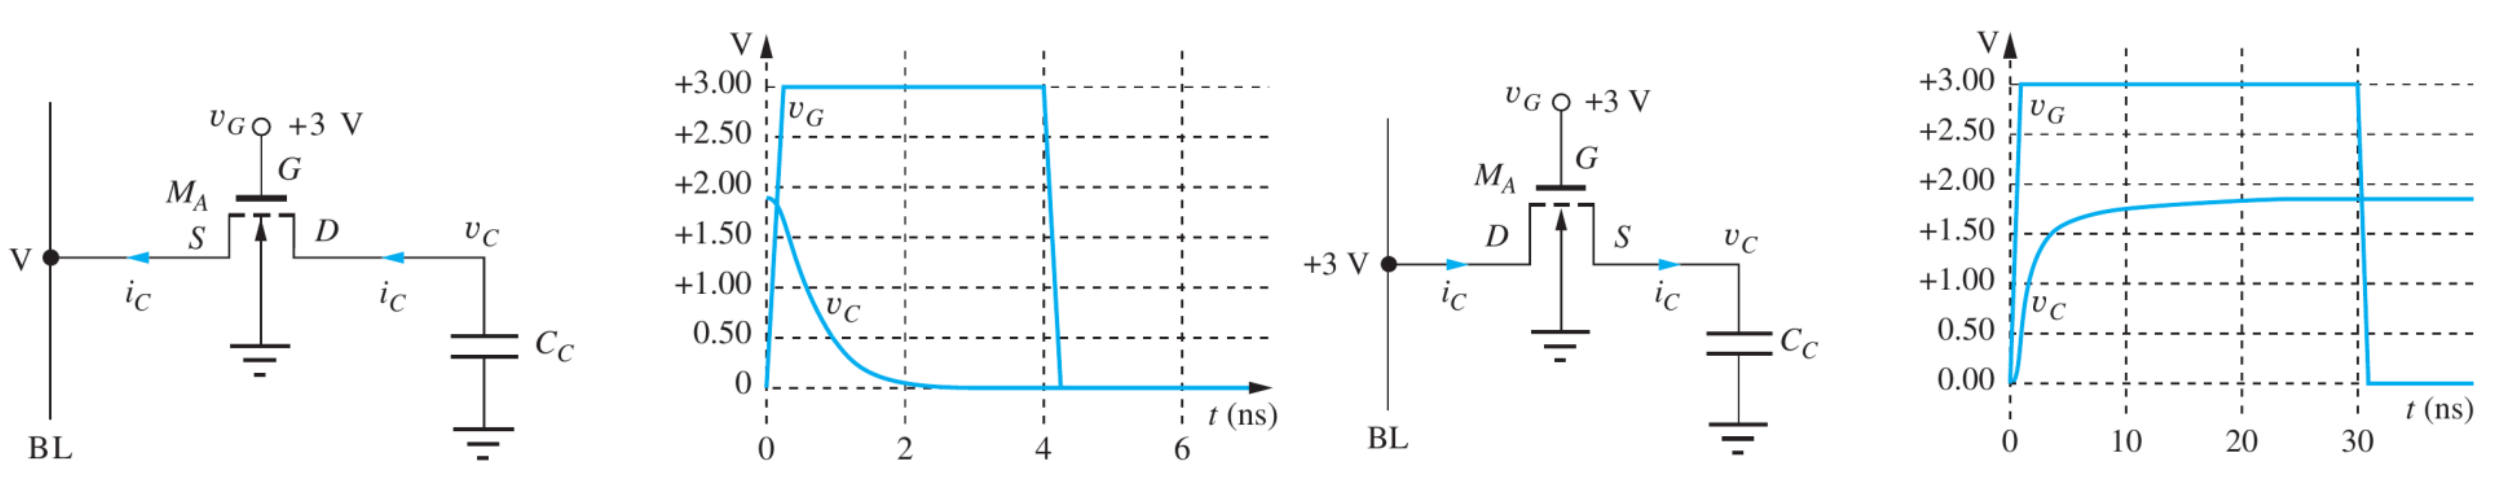
\includegraphics[width=1\linewidth]{img/ram_dinamica.png}
\end{figure}

Anche in questo caso abbiamo lo stesso problema dato che viene utilizzato un pass-transistor: non arriviamo al valore di tensione della bitline bensì sarà minore, come si può vedere dal grafico Spice di destra. Per far arrivare a 3V il condensatore basta mettere ad esempio $V_G = 5V$,la tensione sulla bitline lasciarla invariata e sul condensatore avremo il valore desiderato. Ecco il perché delle varie tensioni che vi sono sulla scheda madre: $3V$, $5V$, $12V$.

\subsection{Lettura e Scrittura}

In questo caso, a differenza delle celle statiche, non c'è un inverter che pilota la bitline, ma c'è appunto il condensatore che da solo deve far in modo di variare abbastanza la bitline per leggere il valore correttamente. La bitline invece è realmente raffigurabile come un condensatore molto grosso.


\begin{figure}[htbp]
    \centering
    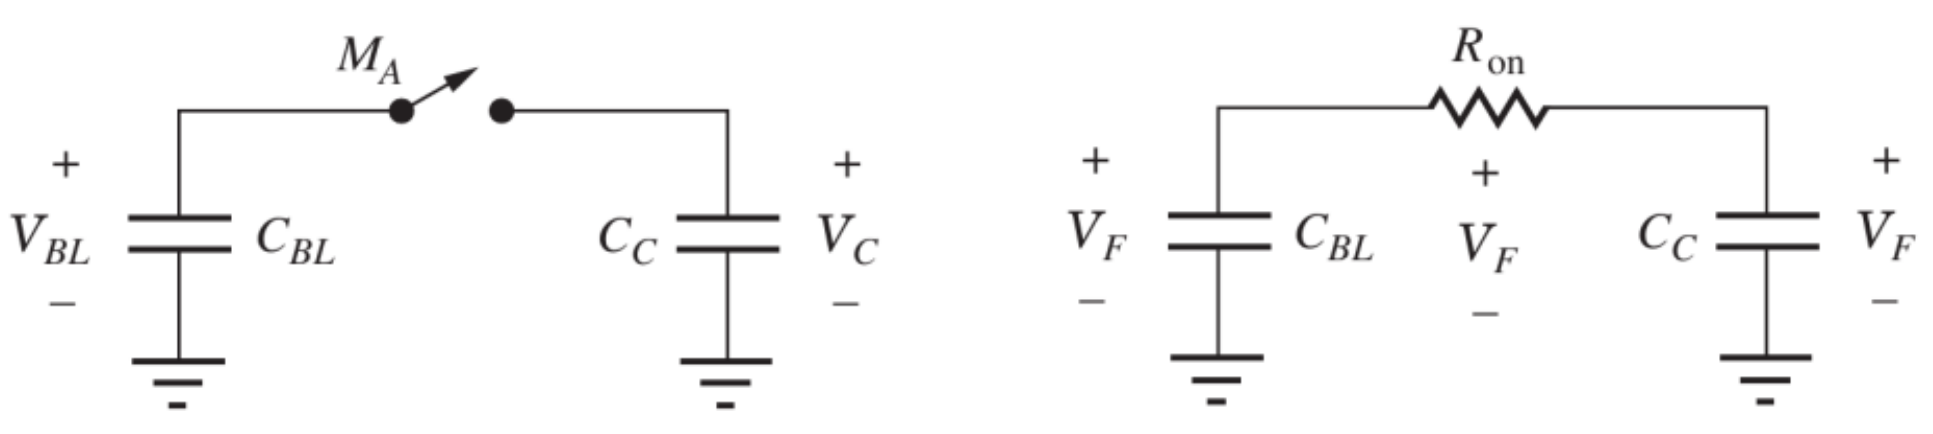
\includegraphics[width=0.65\linewidth]{img/cella_rammona.png}
\end{figure}

\newpage
Come prima si carica a metà, della tensione immagazzinata nel condensatore, il valore della bitline. Per leggere il valore chiudiamo l'interruttore, attivando il transistore di accesso. A questo punto abbiamo un circuito costituito dai due condensatori e da una resistenza equivalente $R_{on}$ data dal condensatore stesso.  

A fronte ci ciò, si avvierà un trasferimento di carica da una parte all'altra a seconda se il condensatore sia carico o meno, fino a quando le tensioni si equivalgono. Quindi calcolando la carica iniziale e finale, possiamo definire il valore.

\paragraph{}
La carica iniziale è data da:

\begin{equation*}
    Q_I = C_CV_C + C_{BL}V_{BL}
\end{equation*}
\begin{equation*}
    Q_F = (C_C + C_{BL})V_{F}
\end{equation*}
\begin{equation*}
    Q_I = Q_F
\end{equation*}
\begin{equation*}
    V_F = \frac{ C_CV_C + C_{BL}V_{BL}}{C_C + C_{BL}}
\end{equation*}
Se $C_{BL} >> C_C$, allora $V_F \approx	V_{BL}$ ed il calore $C_C$ va praticamente perso. Quindi la tensione finale cambia di pochissimo e per rilevarla occorre un sense amplifier molto sensibile per rilevare la variazione di $V_{BL}$


\paragraph{Esempio:}
 \begin{itemize}
     \item[] $C_{BL} = 49 C_C$
     \item[] $ V_0 = 0V$ e $V_1 = 2V$
 \end{itemize}
precarichiamo la $V_{BL} = 1V$, il valore finale risulterà:

\begin{equation*}
    V_F = \frac{ C_CV_C + C_{BL}V_{BL}}{C_C + C_{BL}} = \frac{ C_CV_C + 49 C_CV_{BL}}{C_C + 49 C_C} = \frac{V_C+49\cdot1}{50} = \frac{1}{50V_C} + \frac{49}{50}
\end{equation*}

Dunque:

\begin{itemize}
    \item[] se $V_C = 0V$, allora $V_F = 0.98V$
    \item[] se $V_C = 2V$, allora $V_F = 1.02V$
\end{itemize}

Lo scarto è di soli $20mV$, il sense amplifier porta la bitline al valore finale, e riscrive anche il valore nella cella, perché è andato perso, vi è un refresh dell'intera riga implicito.

Una volta letta la riga, non c'è bisogno di rileggerla, bensì si salverà il dato in un vero flip-flop con anello di feedback.

\newpage
\chapter{Sense amplifier}
Questo dispositivo funziona esattamente come un latch posto in una situazione di equilibrio instabile e vogliamo che la cella lo faccia cadere da una parte o dall'altra a seconda del suo contenuto.

\begin{figure}[htbp]
    \centering
    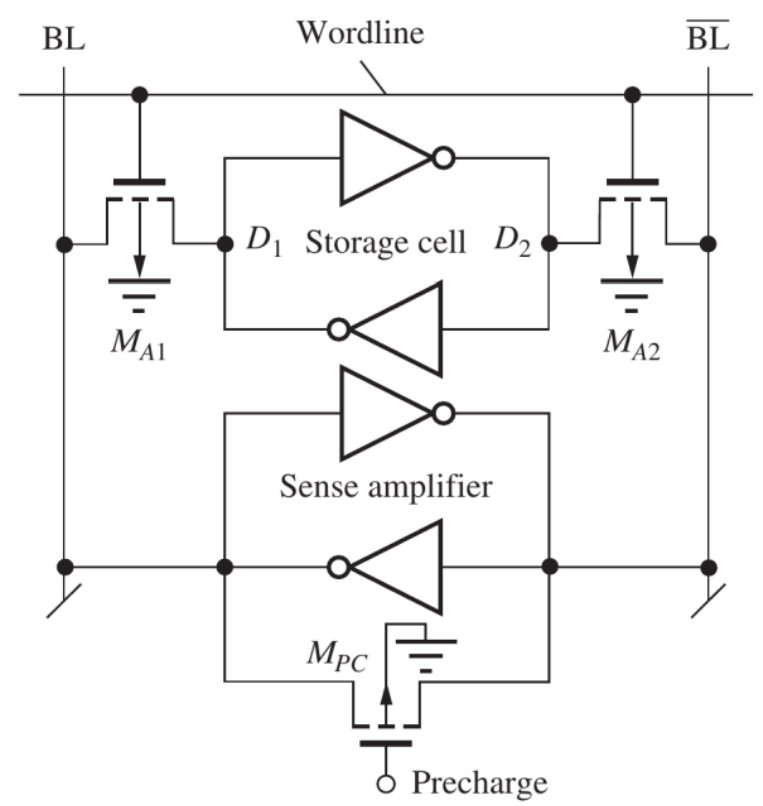
\includegraphics[width=0.4\linewidth]{img/Sense_amp.png}
    \caption{Sense amplifier}
\end{figure}

\section{Precarica e lettura}

Per raggiungere questo punto si imposta il valore, sia a destra che a sinistra, alla stessa tensione che si imposta sulla BL, ovvero metà della tensione di lavoro. Dopo aver caricato il valore si stacca il precharge, si attiva la wordline, la cella fa variare le bitlines e il sense amplifier porta effettivamente al valore finale dato che è nel punto di equilibrio instabile, il quale amplifica questa variazione dato che i suoi transistori possiamo farli grossi, ce lo possiamo permettere perché sono posti solo sulle colonne.


\begin{figure}[htbp]
    \centering
    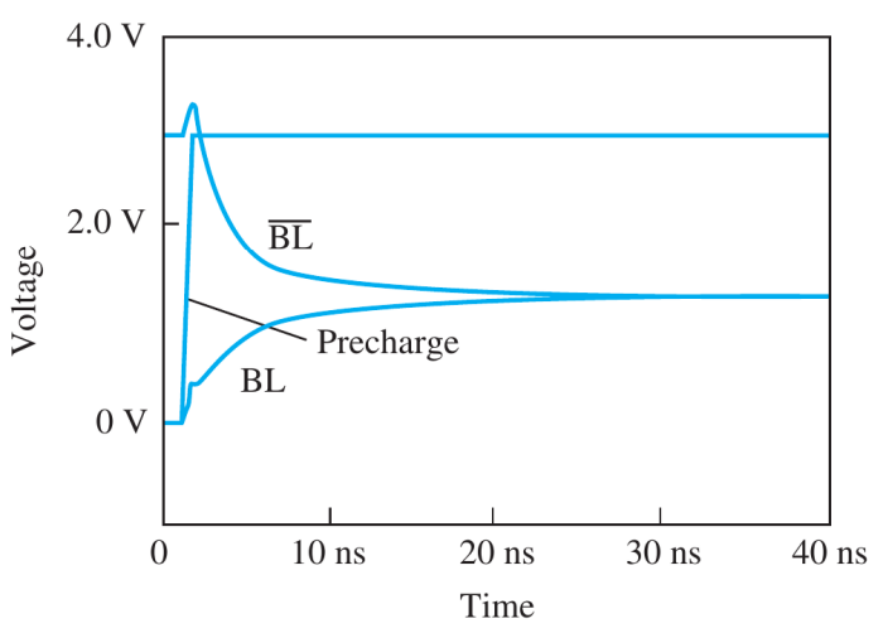
\includegraphics[width=0.5\linewidth]{img/prcaroca.png}
    \caption{Precarica delle bitlines}
\end{figure}

\newpage
\section{Consumi}

Consumi significativi in fase di precarica, i due inverter nel sense amplifier, i gate sono posti a $V_{DD}/2$, dunque entrambi i transistori conducono nella fase di precarica con un conseguente passaggio di corrente e consumo statico.



\section{Row Decoders}

I decoder CMOS generalmente sono troppo grossi, infatti MOS a rapporto, sia con porte NOR
(uscita attiva alta), sia con porte NAND (uscita attiva bassa). Attenzione però ai consumi!

Dal punto di vista dei consumi è meglio utilizzare delle porte NAND, e per ottenere l'uno in uscita basta metterci un inverter. Il problema che i transistori sono in serie il che comporta un circuito più lento.

\begin{figure}[htbp]
    \centering
    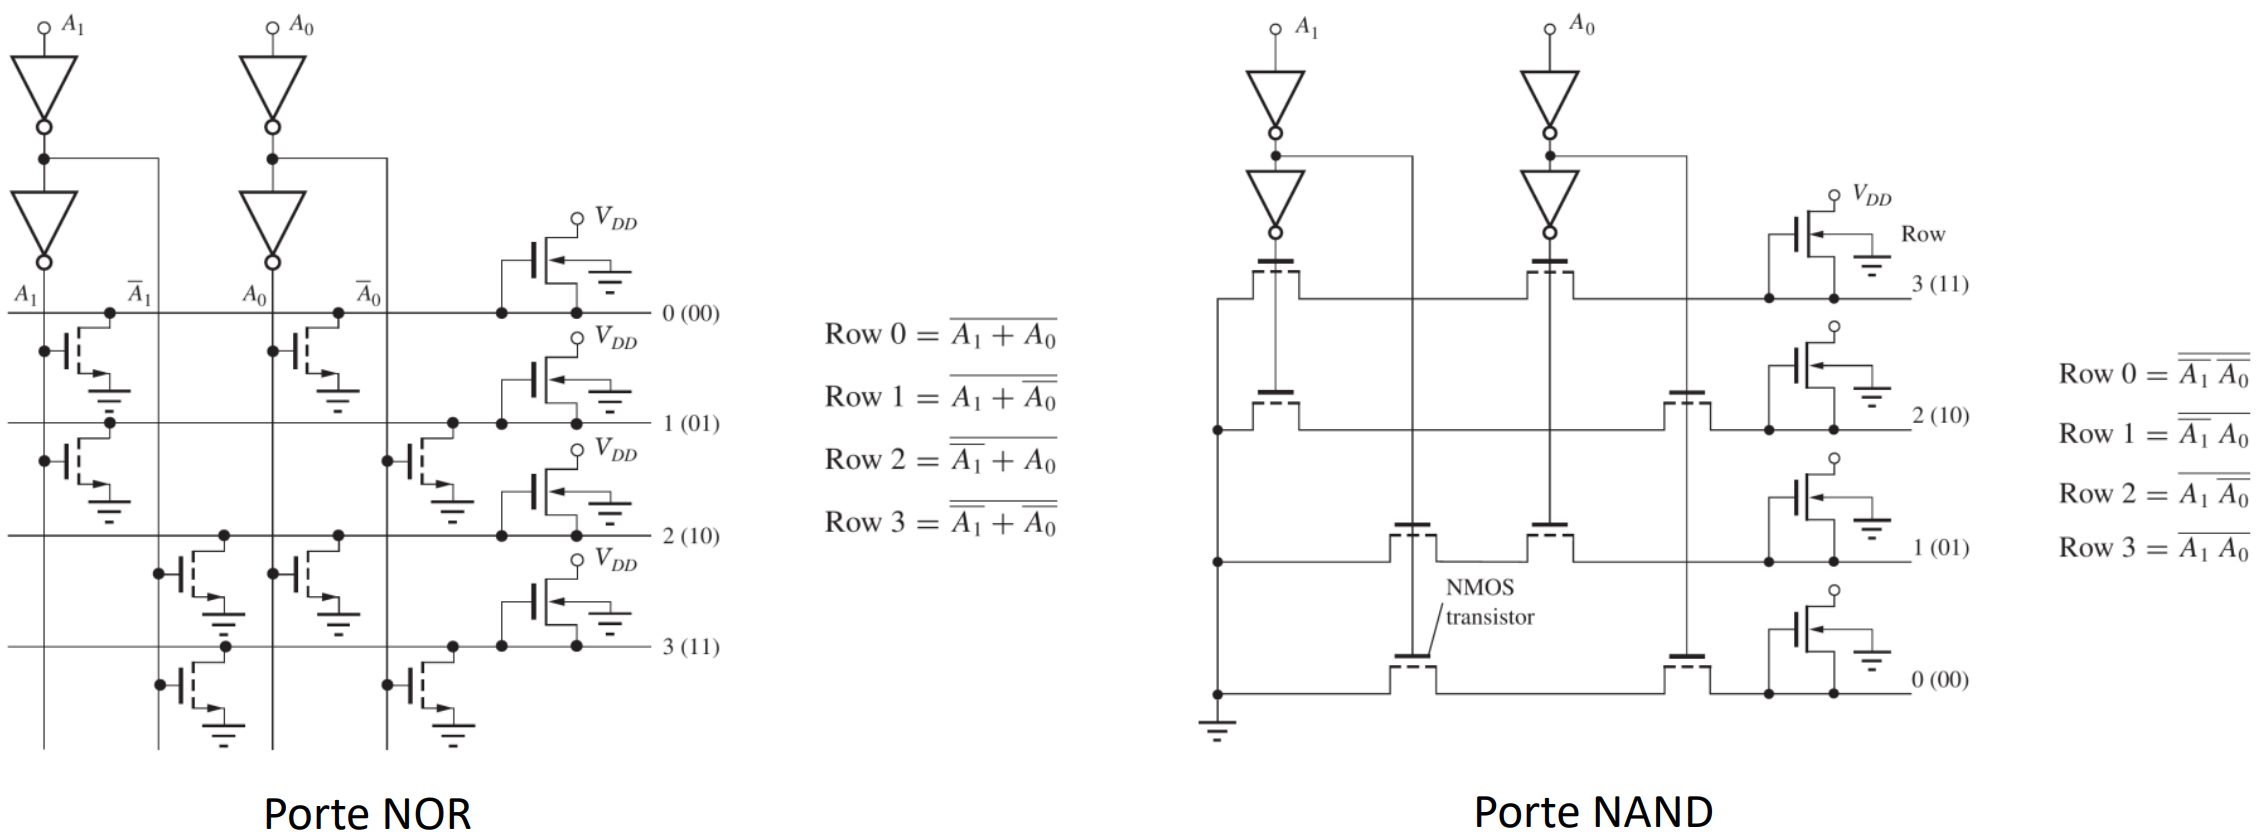
\includegraphics[width=1\linewidth]{img/row_dec.png}
    \caption{Row Decoders}
\end{figure}

Questa figura rappresenta una decodifica in binario da 2 bit a 4 bit, vogliamo che solo una bit dei 4 valga 1.


\newpage
\section{Column Decoders}

Questa decodifica di colonna non è altro che un multiplexer. La sua realizzazione può essere realizzata tramite CMOS ma diventa troppo onerosa per vie delle risorse. Altre soluzioni possono essere quella di usare transmission gate o pass transistor.

\begin{figure}[htbp]
    \centering
    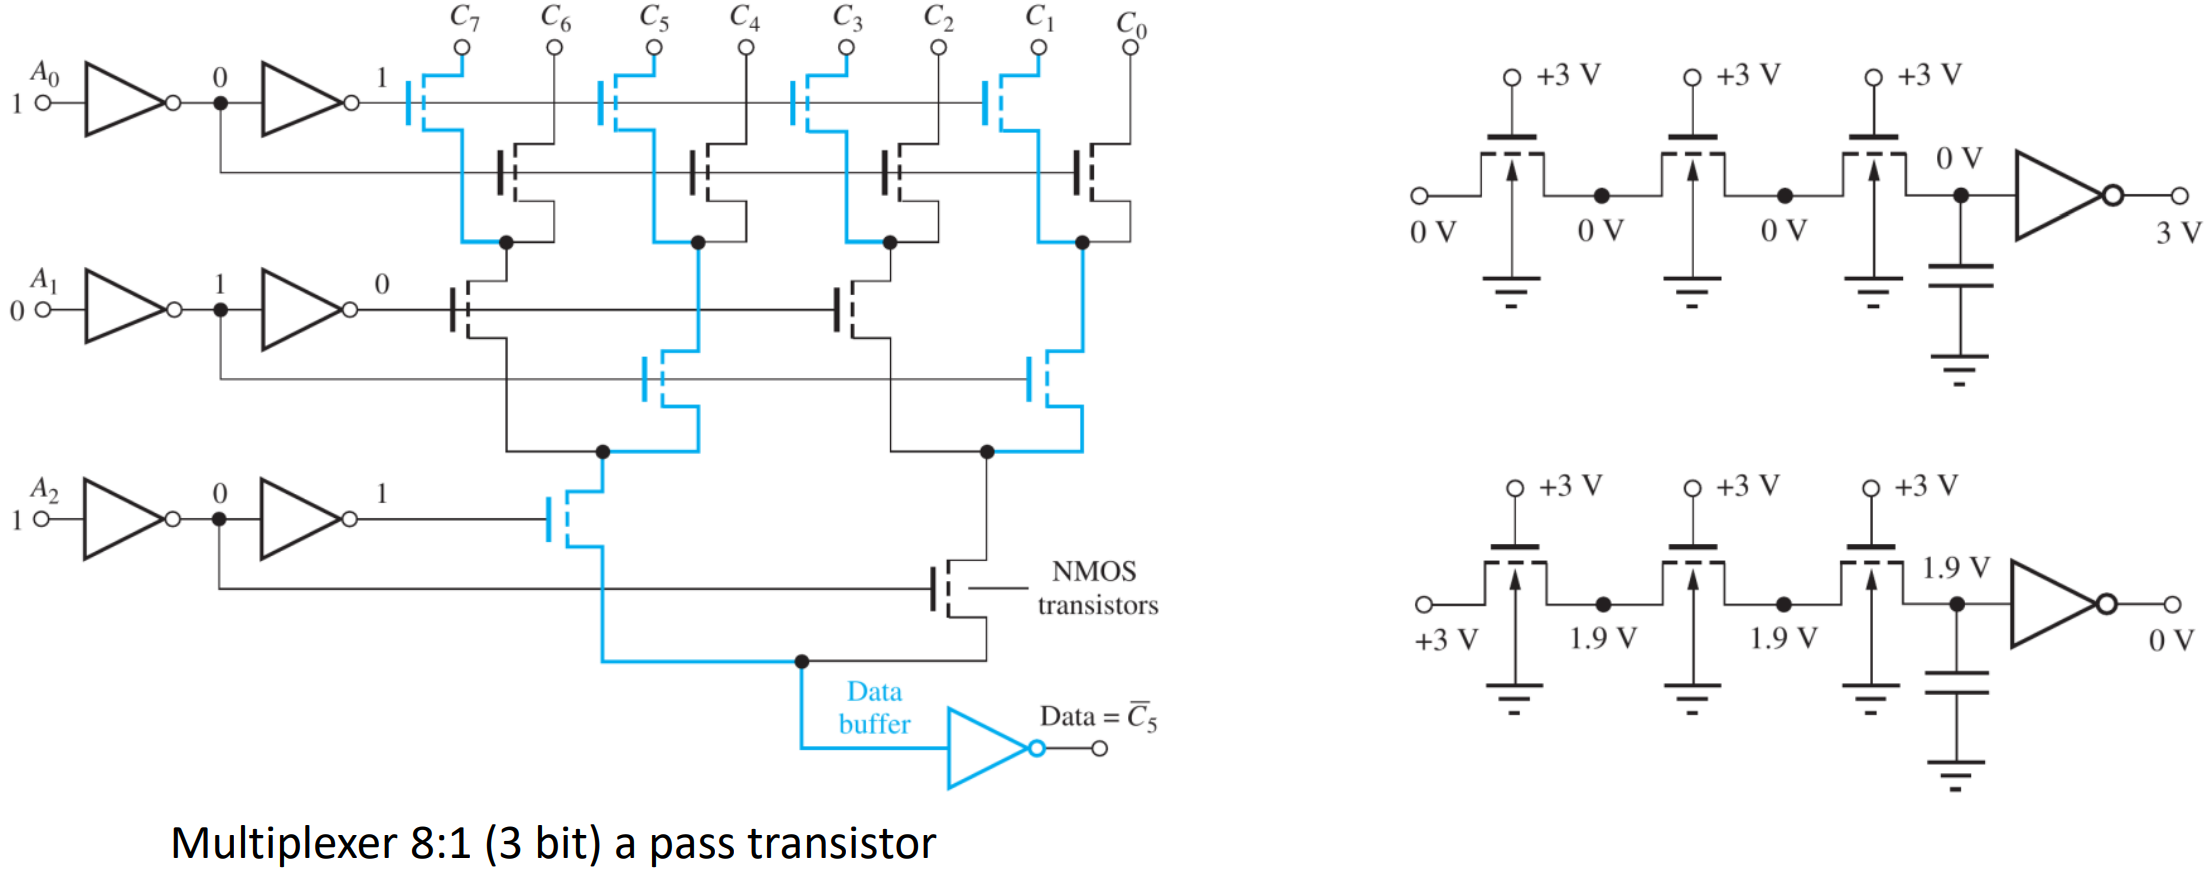
\includegraphics[width=1\linewidth]{img/colum_dec.png}
    \caption{Column Decoders}
\end{figure}

